%!TEX root = report.tex
In this section we present and discuss some of the experiments we have performed with our simulation. Each experiment in this section was performed on a grid of 1200 particles, with the spring constants sampled from a normal distribution with a mean of 0 and a standard deviation of 0.99. The seed was reset to the same value at the start of each simulation, consequently all initial grids have the same spring constants. When a number of springs under the highest strain where broken, we broke 97 springs at each step. When the second method was used, we broke the springs with a strain greater than $1.04$. % If springs were stretched $\vartheta = 0.1$.

Below we discuss the possible combinations of breaking versus stretching and the different conditions under which springs are either broken or stretched. Lastly we review the parameters that influence the breaking and stretching of springs.

% Break x with highest strain
	\begin{figure*}
		\centering
		%!TEX root = report.tex	
\begin{subfigure}{0.16\textwidth}
	\centering
	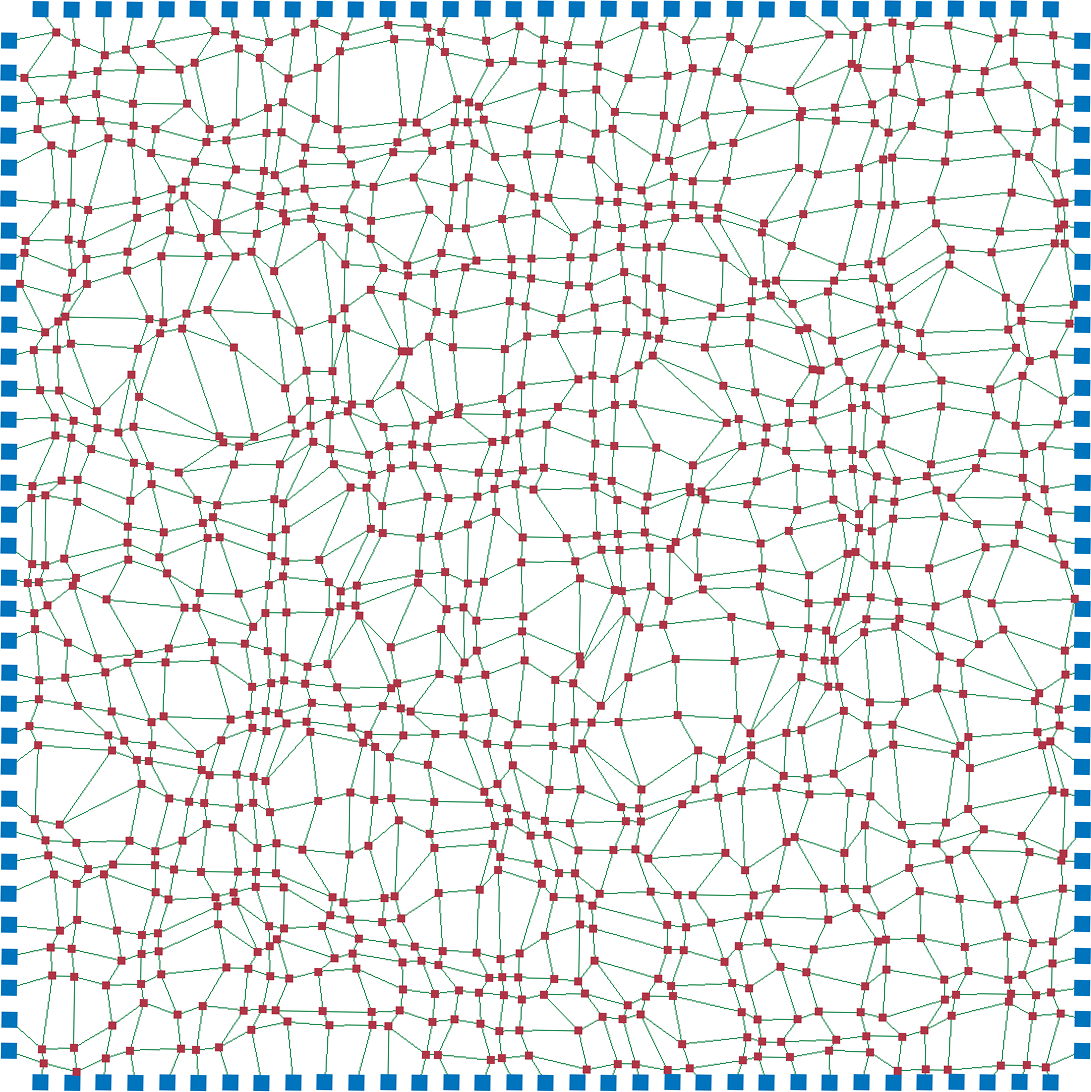
\includegraphics[
		width=\textwidth, 
		height=\textwidth, 
		keepaspectratio=true]
	{./img/results/1200_0_1_highest_97_step_0}
	\caption{Step 0}
	\label{fig:experiment:highestStrain:0}
\end{subfigure}
\begin{subfigure}{0.16\textwidth}
	\centering
	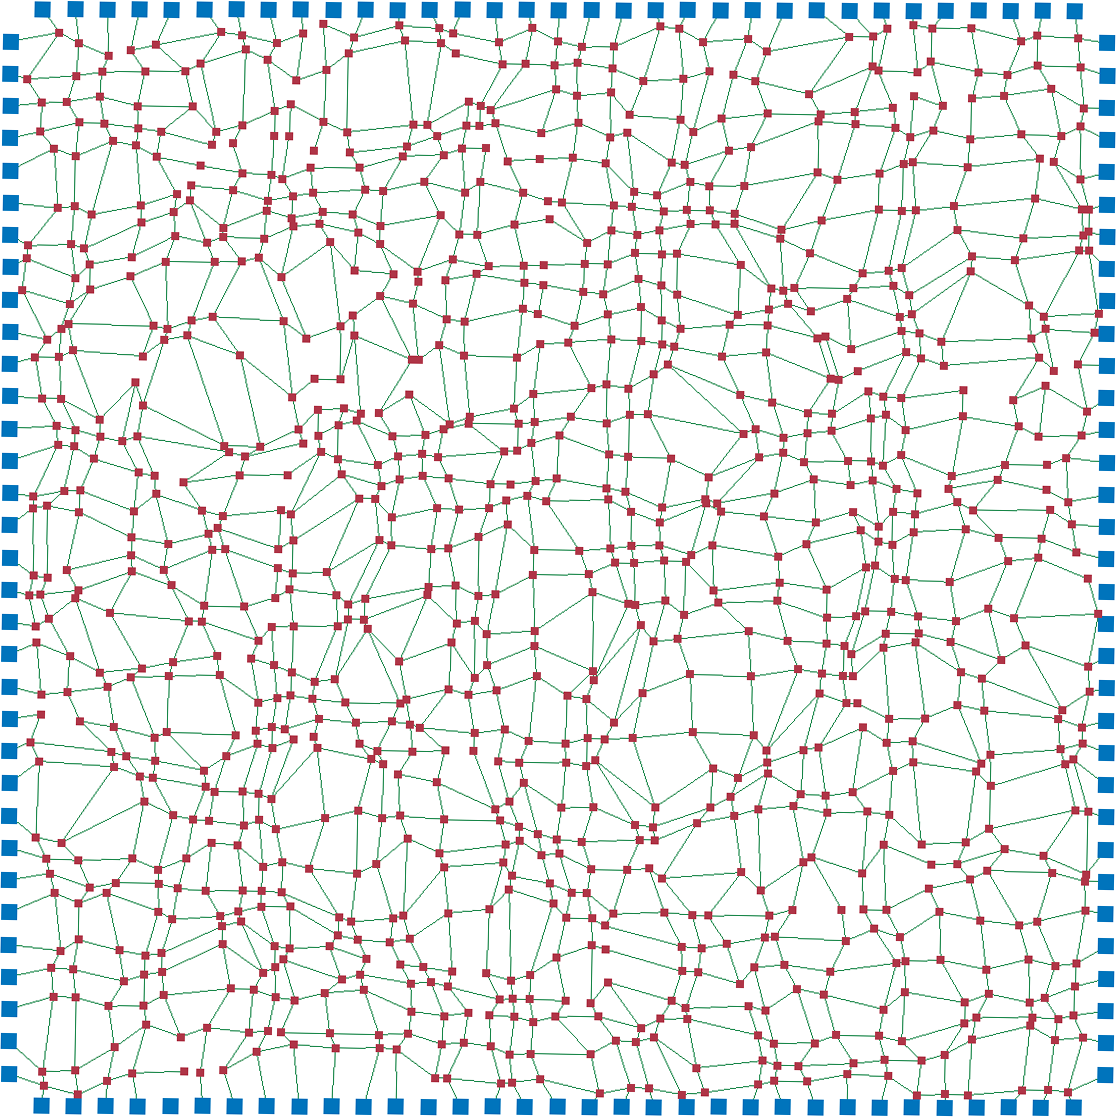
\includegraphics[
		width=\textwidth, 
		height=\textwidth, 
		keepaspectratio=true]
	{./img/results/1200_0_1_highest_97_step_1}
	\caption{Step 1}
	\label{fig:experiment:highestStrain:1}
\end{subfigure}	
\begin{subfigure}{0.16\textwidth}
	\centering
	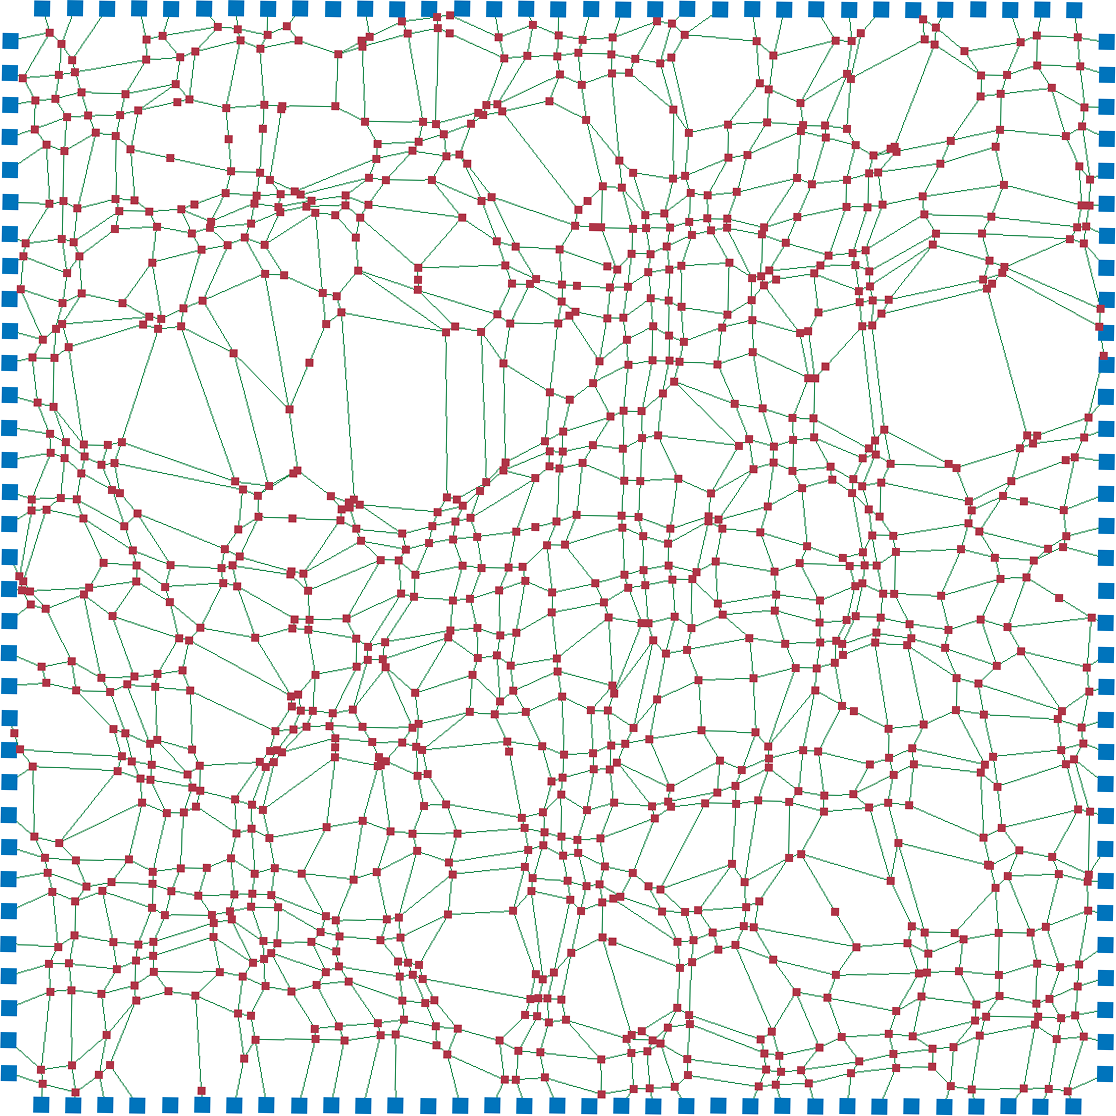
\includegraphics[
		width=\textwidth, 
		height=\textwidth, 
		keepaspectratio=true]
	{./img/results/1200_0_1_highest_97_step_2}
	\caption{Step 2}
	\label{fig:experiment:highestStrain:2}
\end{subfigure}		
\begin{subfigure}{0.16\textwidth}
	\centering
	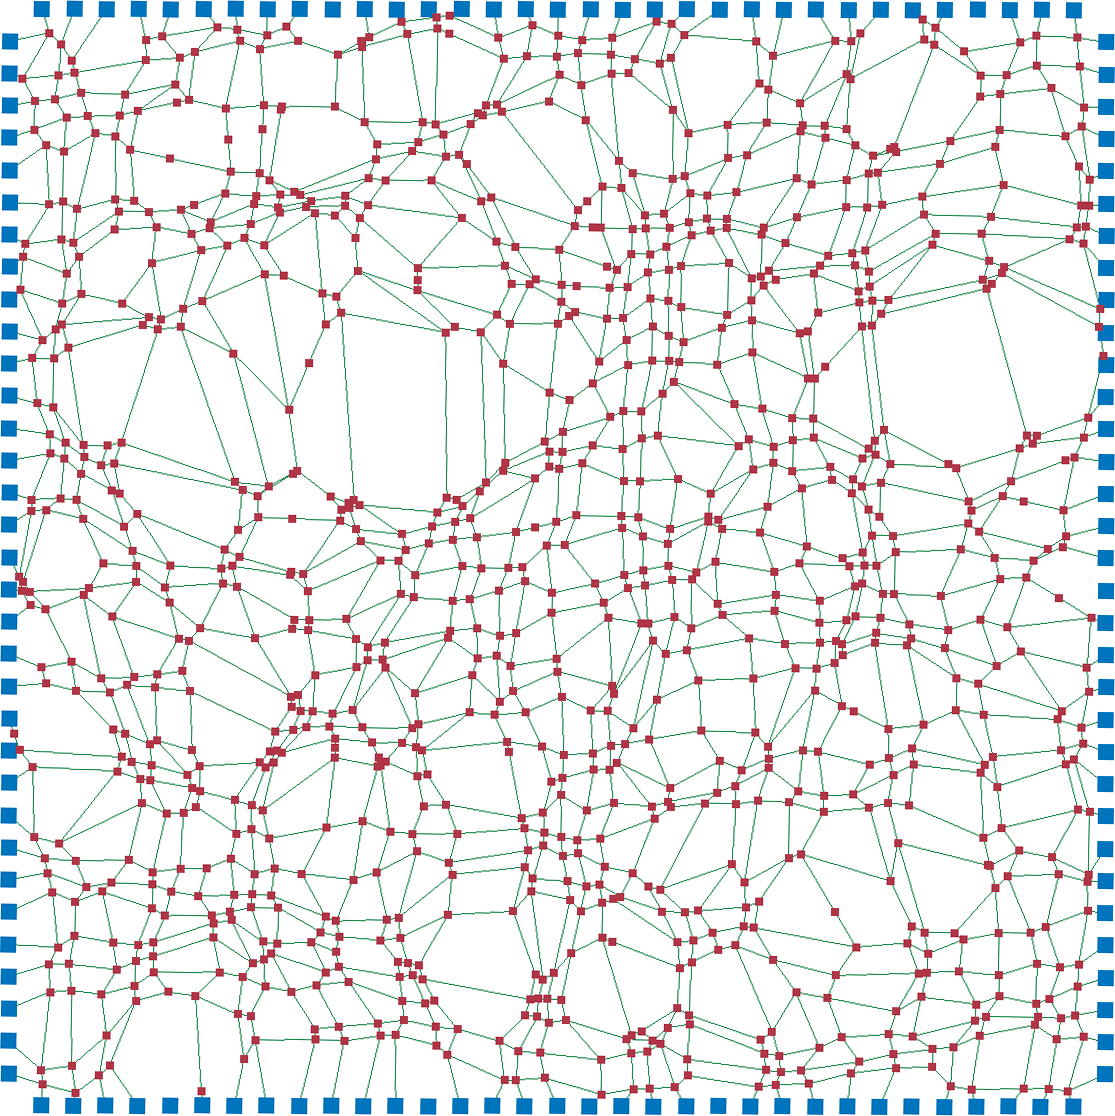
\includegraphics[
		width=\textwidth, 
		height=\textwidth, 
		keepaspectratio=true]
	{./img/results/1200_0_1_highest_97_step_3}
	\caption{Step 3}
	\label{fig:experiment:highestStrain:3}
\end{subfigure}			
\begin{subfigure}{0.16\textwidth}
	\centering
	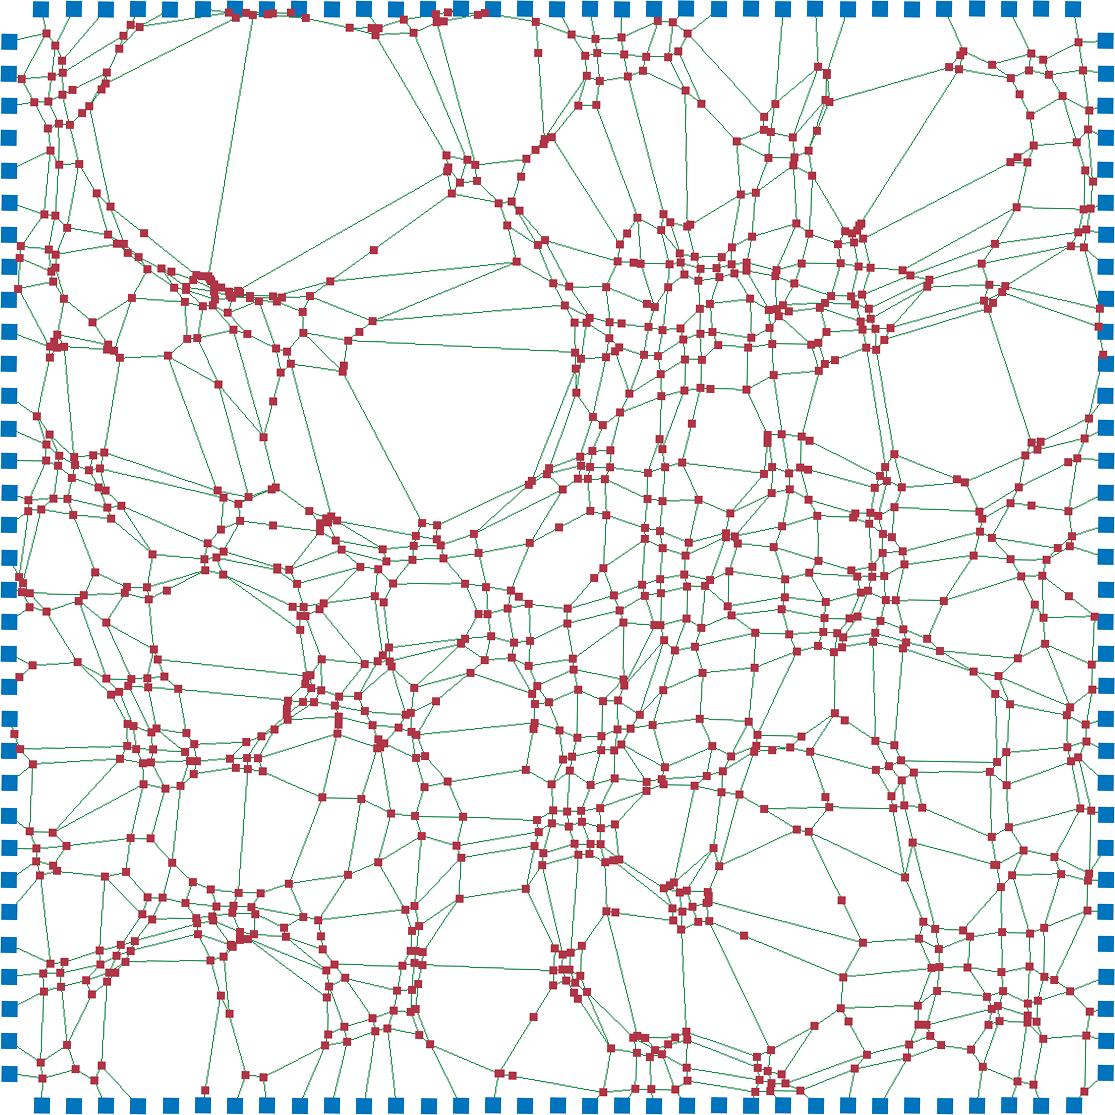
\includegraphics[
		width=\textwidth, 
		height=\textwidth, 
		keepaspectratio=true]
	{./img/results/1200_0_1_highest_97_step_4}
	\caption{Step 4}
	\label{fig:experiment:highestStrain:4}
\end{subfigure}				
\begin{subfigure}{0.16\textwidth}
	\centering
	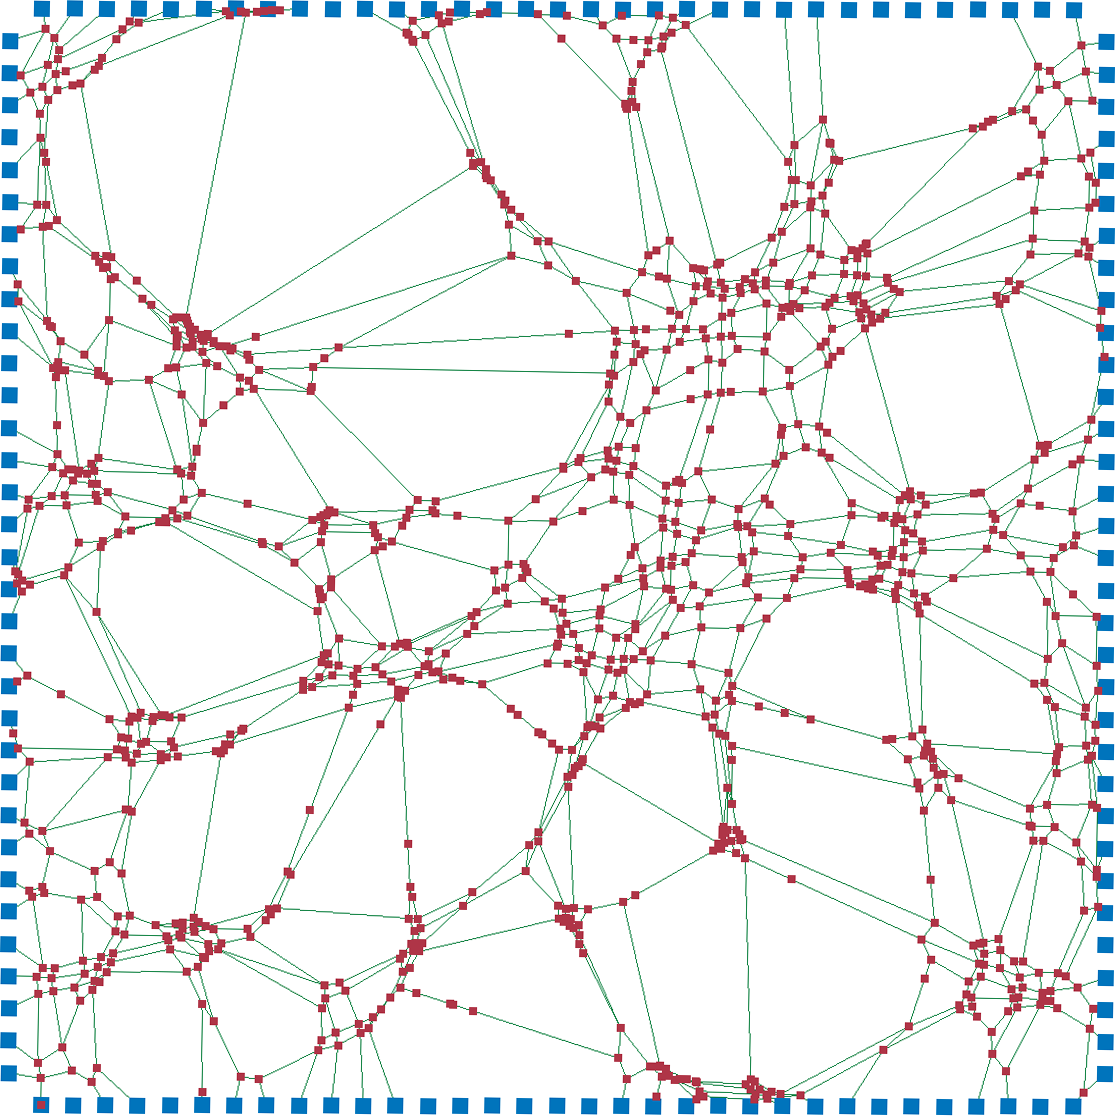
\includegraphics[
		width=\textwidth, 
		height=\textwidth, 
		keepaspectratio=true]
	{./img/results/1200_0_1_highest_97_step_5}
	\caption{Step 5}
	\label{fig:experiment:highestStrain:5}
\end{subfigure}
\begin{subfigure}{0.16\textwidth}
	\centering
	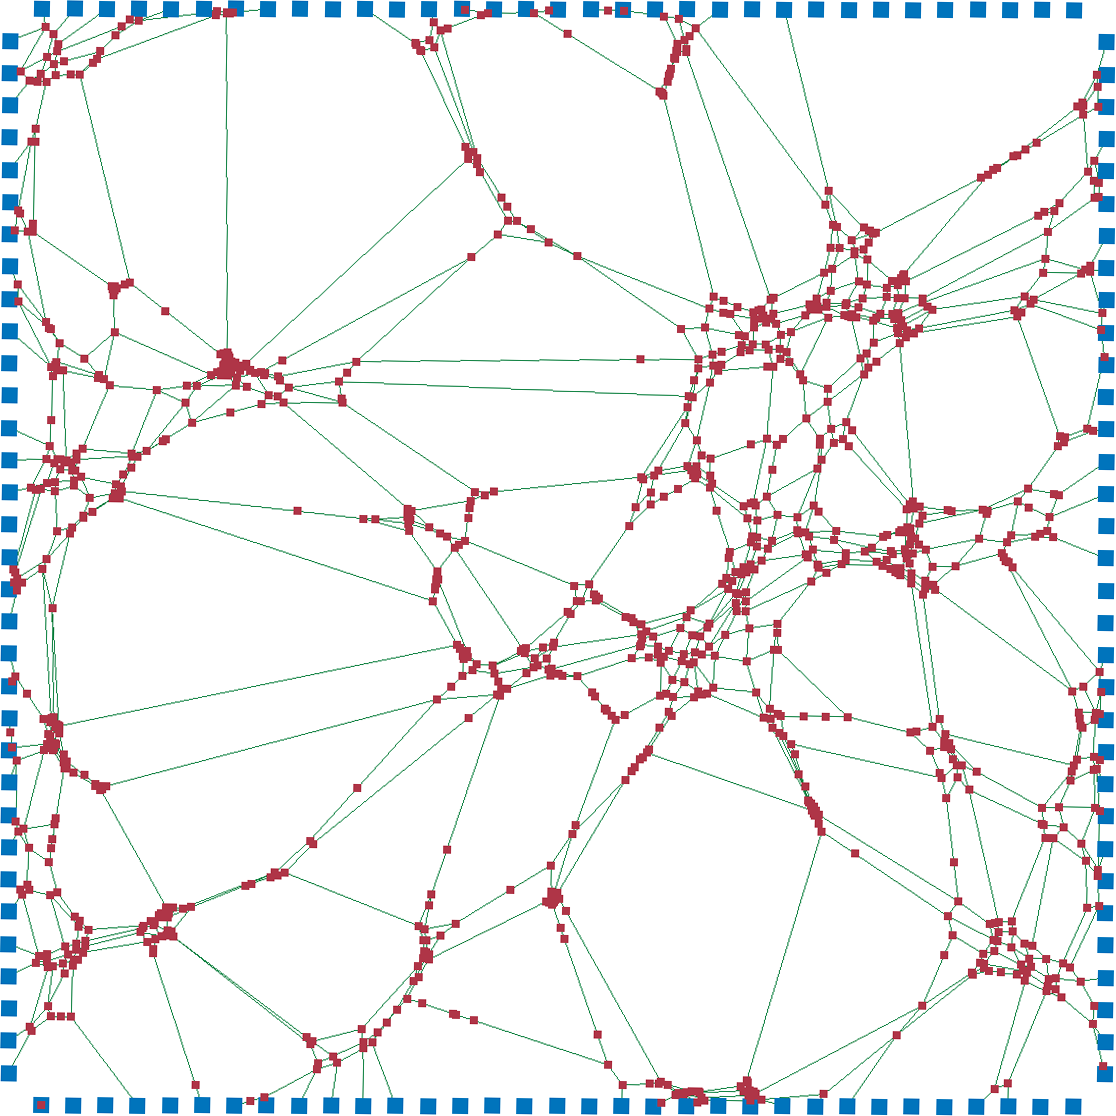
\includegraphics[
		width=\textwidth, 
		height=\textwidth, 
		keepaspectratio=true]
	{./img/results/1200_0_1_highest_97_step_6}
	\caption{Step 6}
	\label{fig:experiment:highestStrain:6}
\end{subfigure}	
\begin{subfigure}{0.16\textwidth}
	\centering
	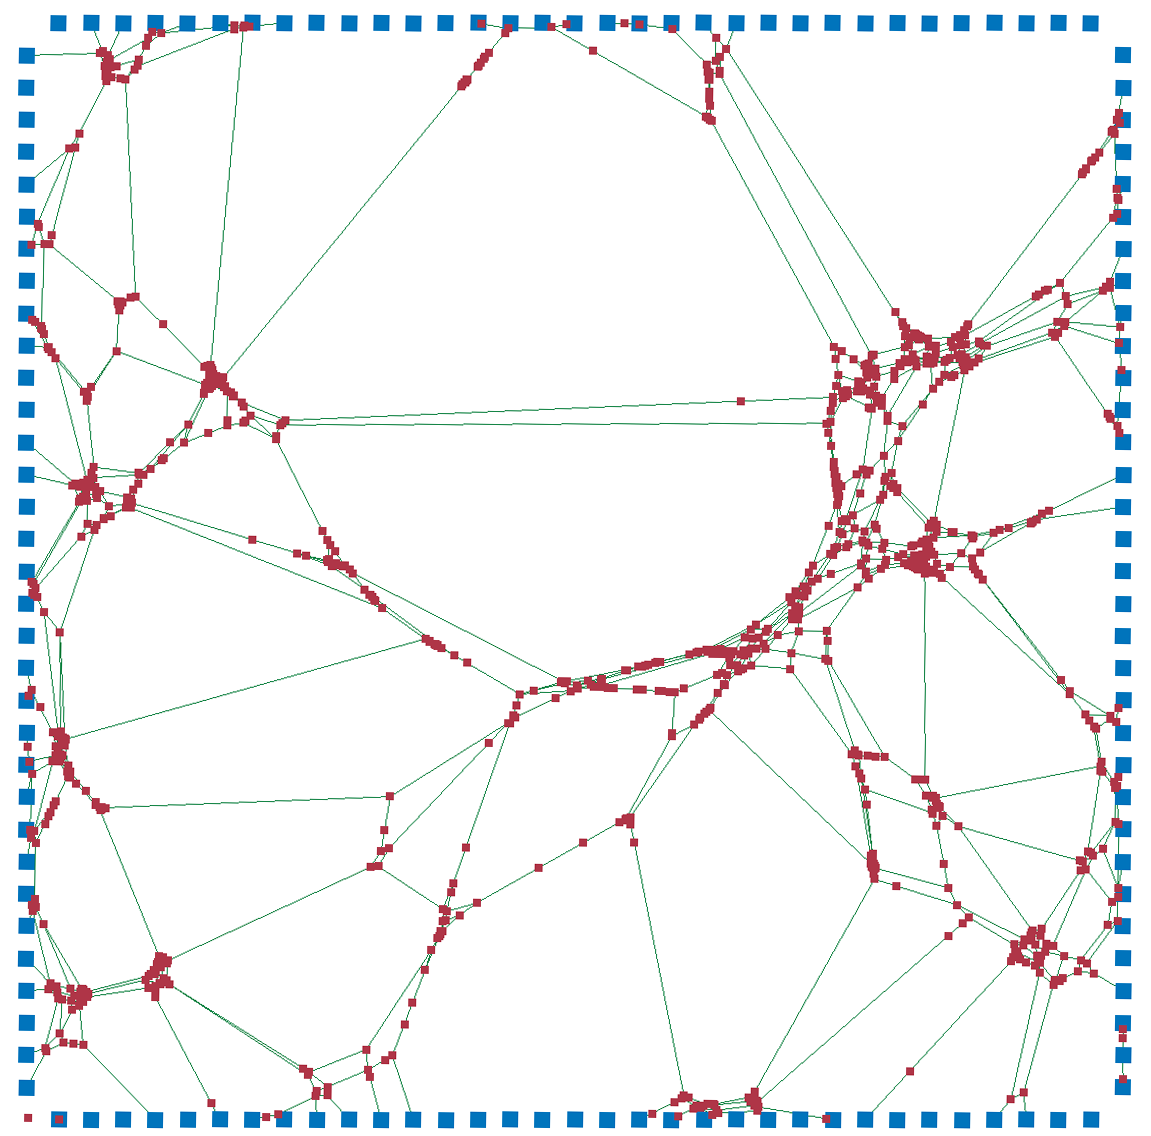
\includegraphics[
		width=\textwidth, 
		height=\textwidth, 
		keepaspectratio=true]
	{./img/results/1200_0_1_highest_97_step_7}
	\caption{Step 7}
	\label{fig:experiment:highestStrain:7}
\end{subfigure}		
\begin{subfigure}{0.16\textwidth}
	\centering
	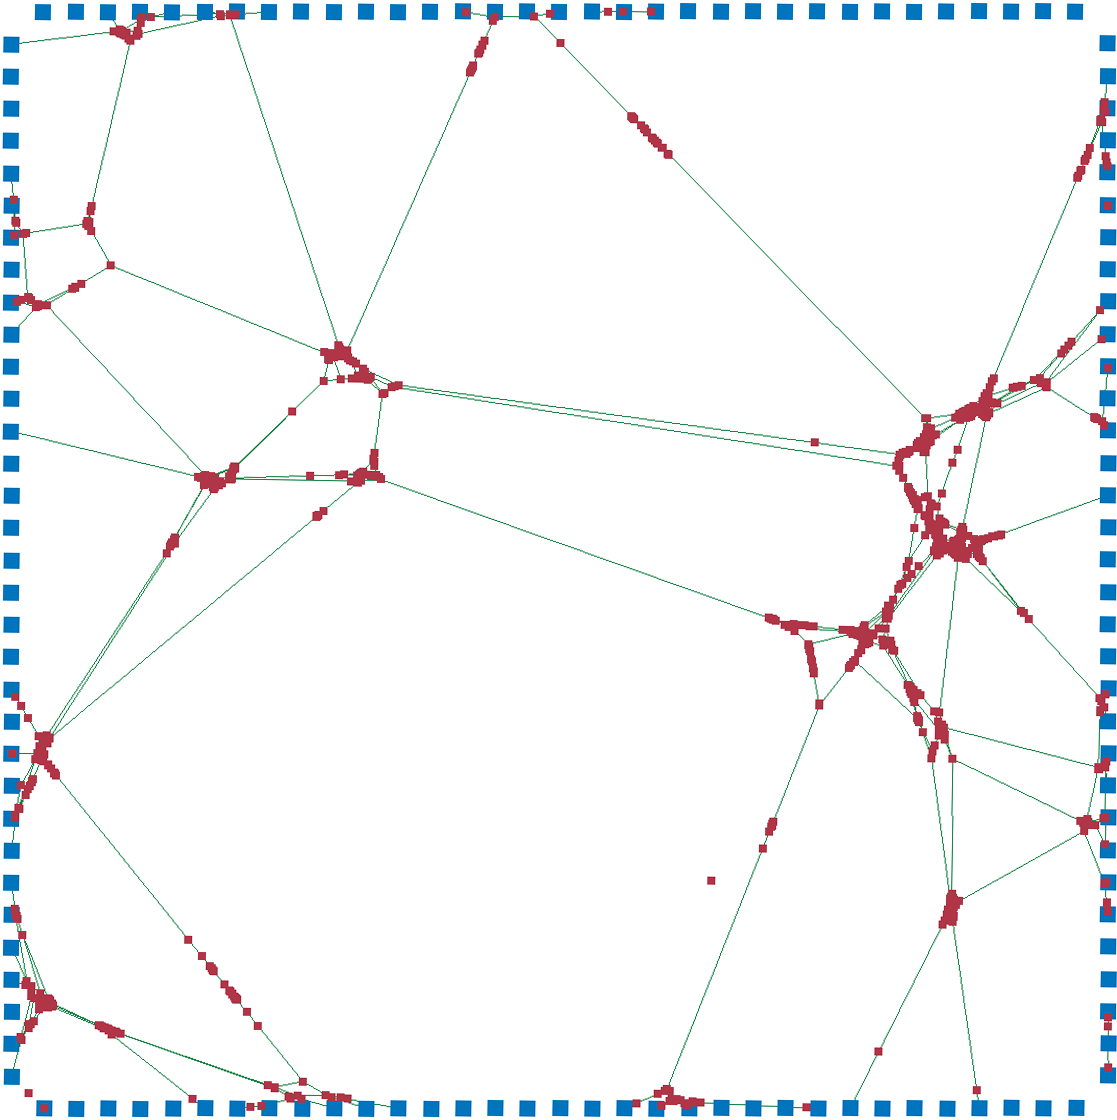
\includegraphics[
		width=\textwidth, 
		height=\textwidth, 
		keepaspectratio=true]
	{./img/results/1200_0_1_highest_97_step_8}
	\caption{Step 8}
	\label{fig:experiment:highestStrain:8}
\end{subfigure}			
\begin{subfigure}{0.16\textwidth}
	\centering
	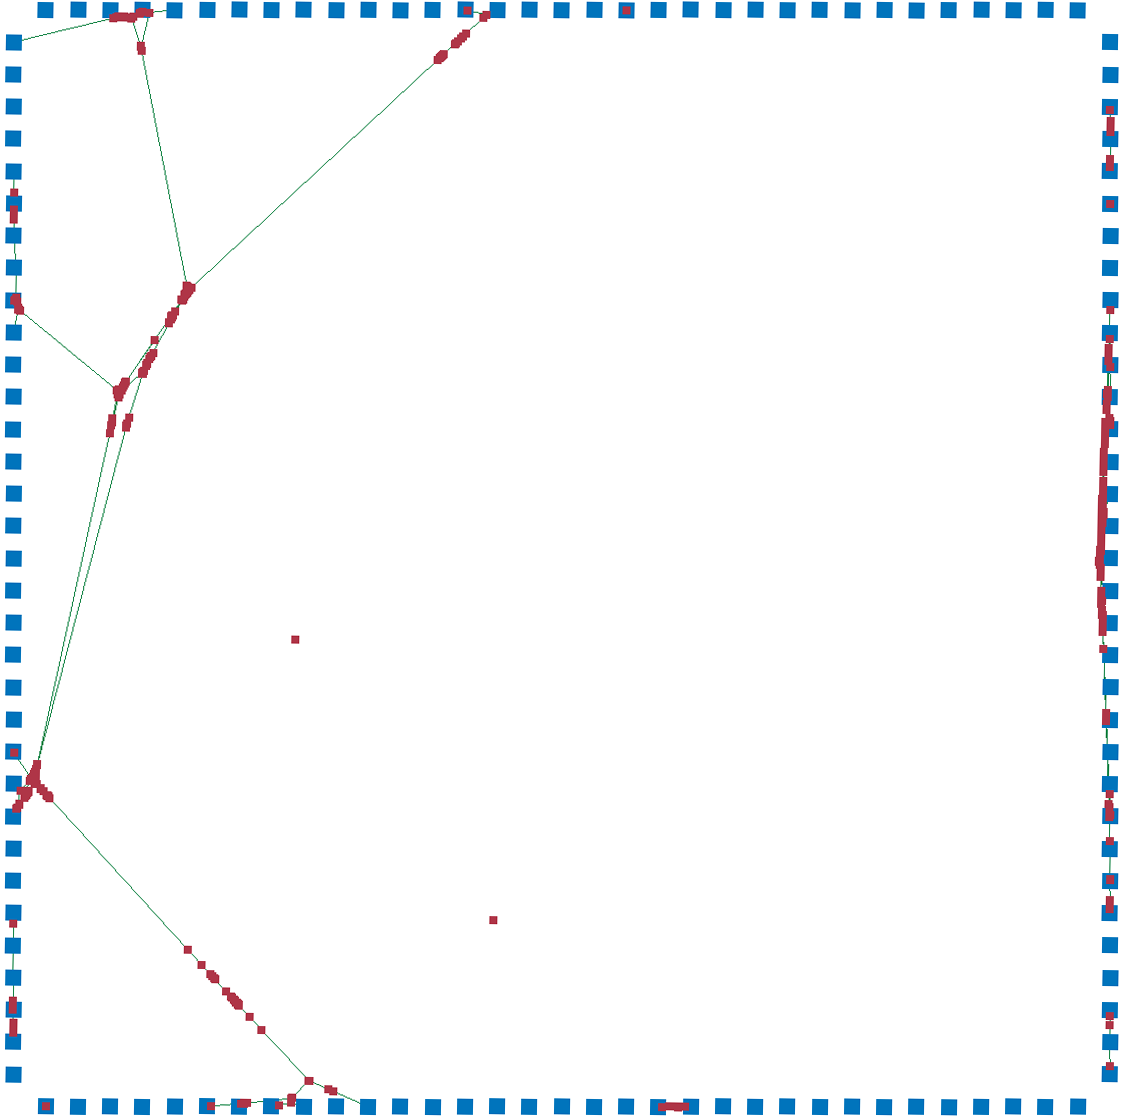
\includegraphics[
		width=\textwidth, 
		height=\textwidth, 
		keepaspectratio=true]
	{./img/results/1200_0_1_highest_97_step_9}
	\caption{Step 9}
	\label{fig:experiment:highestStrain:9}
\end{subfigure}					
\begin{subfigure}{0.16\textwidth}
	\centering
	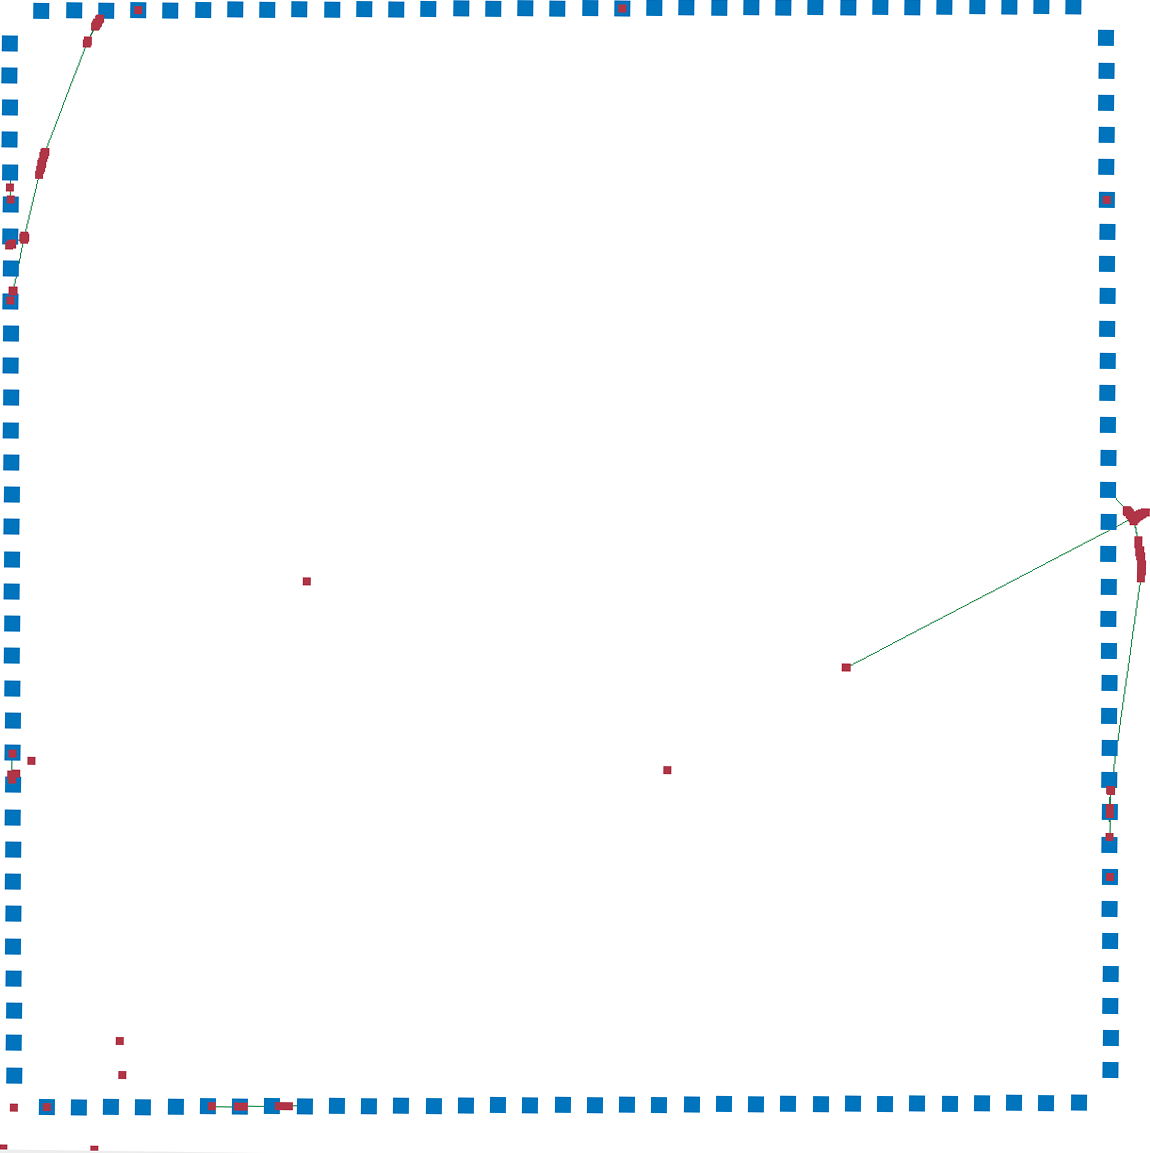
\includegraphics[
		width=\textwidth, 
		height=\textwidth, 
		keepaspectratio=true]
	{./img/results/1200_0_1_highest_97_step_10}
	\caption{Step 10}
	\label{fig:experiment:highestStrain:10}
\end{subfigure}			
\begin{subfigure}{0.16\textwidth}
	\centering
	
\includegraphics[
		width=\textwidth, 
		height=\textwidth, 
		keepaspectratio=true]
	{./img/results/1200_0_1_highest_97_step_11}
	\caption{Step 11}
	\label{fig:experiment:highestStrain:11}
\end{subfigure}						
		\caption{Several steps of the simulation where at each step where springs were broken the 97 springs with the highest strain are broken.}
		\label{fig:experiment:highestStrain}
	\end{figure*}
	\Cref{fig:experiment:highestStrain} presents the results of breaking a number of springs with the highest strain. Initially, \cref{fig:experiment:highestStrain:0,fig:experiment:highestStrain:1}, the pattern resembles cracked mud. However as the simulation progresses the patterns start to resemble a popped balloon, this is especially noticeable in \cref{fig:experiment:highestStrain:6,fig:experiment:highestStrain:7,fig:experiment:highestStrain:8}. When there are no more springs to break the particles have all moved to the lower left corner of the simulation, the point with coordinate $(0,0)$.

% Break x with strain >
	\begin{figure*}
		\centering
		%!TEX root = report.tex	
\begin{subfigure}{0.16\textwidth}
	\centering
	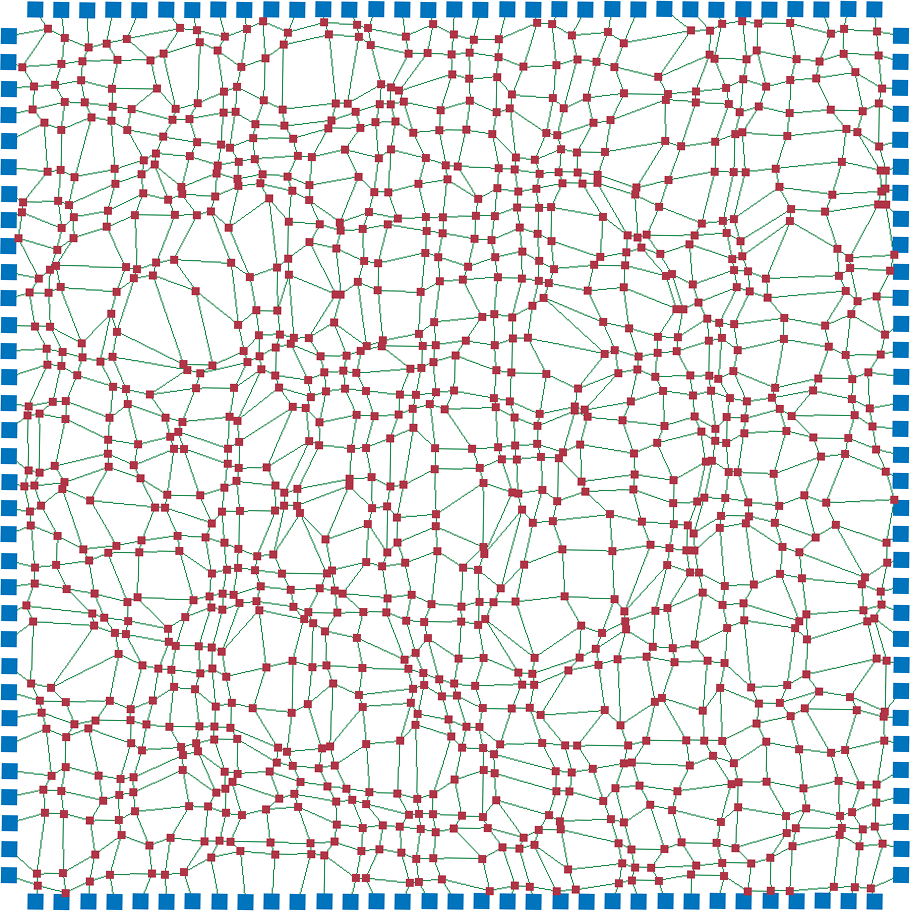
\includegraphics[
		width=\textwidth, 
		height=\textwidth, 
		keepaspectratio=true]
	{./img/results/1200_0_1_greater_104_step_0}
	\caption{}
	\label{fig:experiment:greaterThanStrain:0}
\end{subfigure}
\begin{subfigure}{0.16\textwidth}
	\centering
	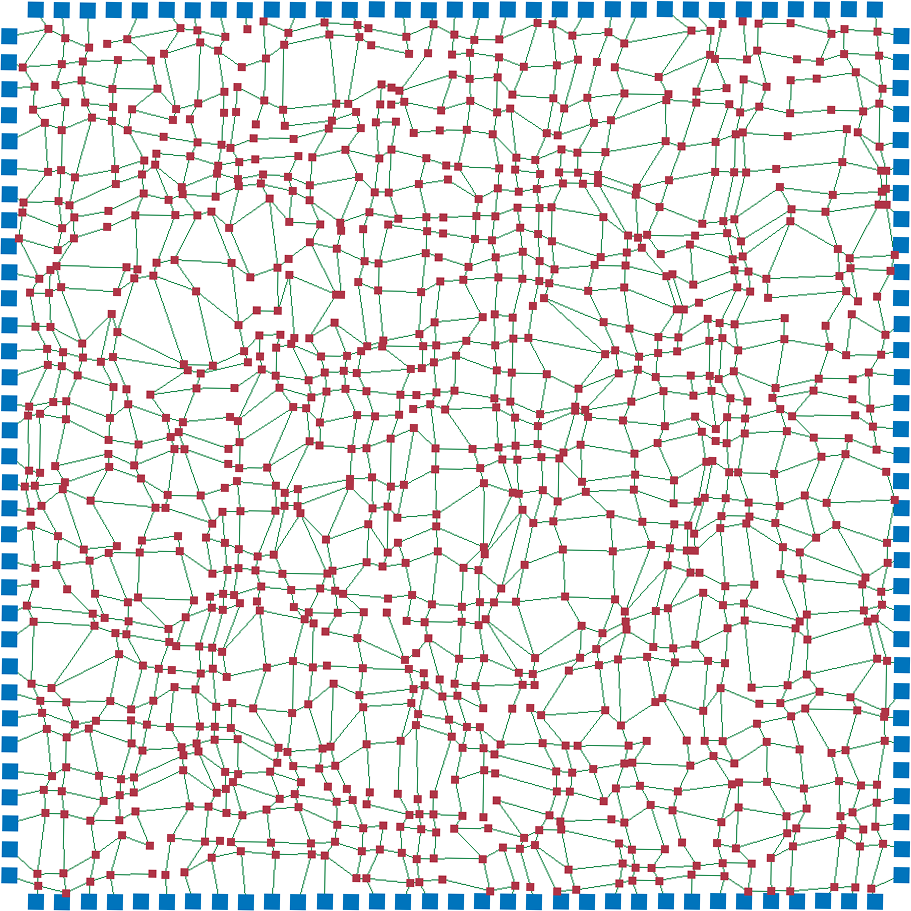
\includegraphics[
		width=\textwidth, 
		height=\textwidth, 
		keepaspectratio=true]
	{./img/results/1200_0_1_greater_104_step_1}
	\caption{}
	\label{fig:experiment:greaterThanStrain:1}
\end{subfigure}	
\begin{subfigure}{0.16\textwidth}
	\centering
	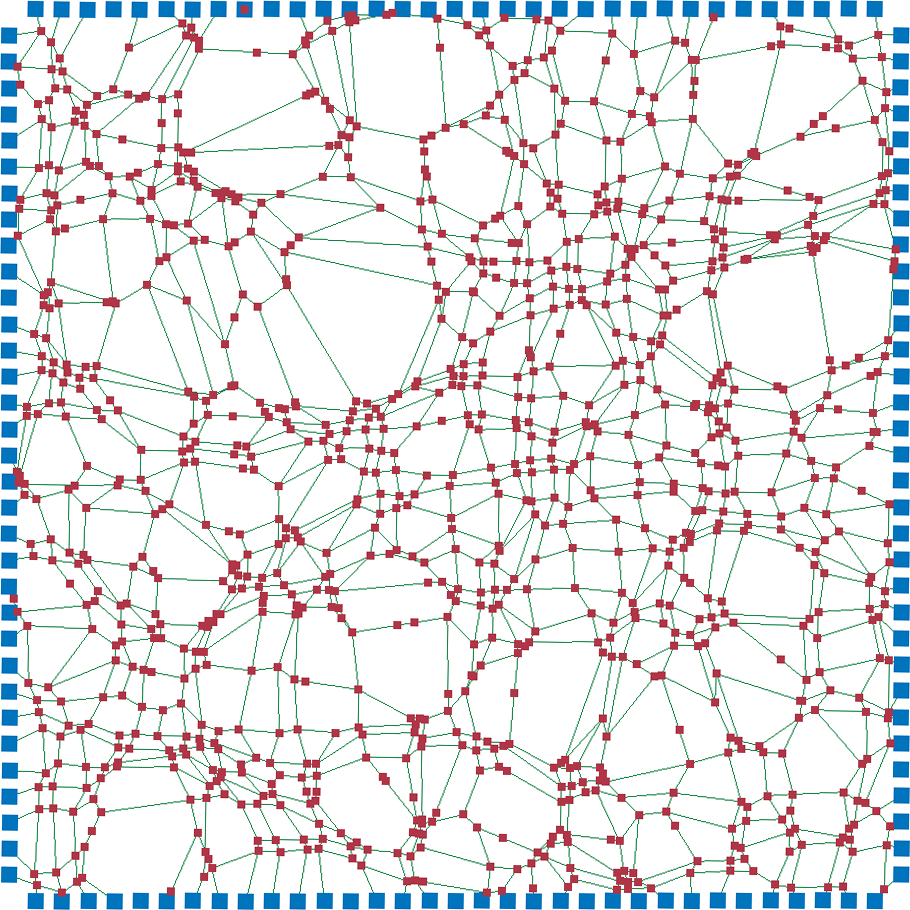
\includegraphics[
		width=\textwidth, 
		height=\textwidth, 
		keepaspectratio=true]
	{./img/results/1200_0_1_greater_104_step_2}
	\caption{}
	\label{fig:experiment:greaterThanStrain:2}
\end{subfigure}		
\begin{subfigure}{0.16\textwidth}
	\centering
	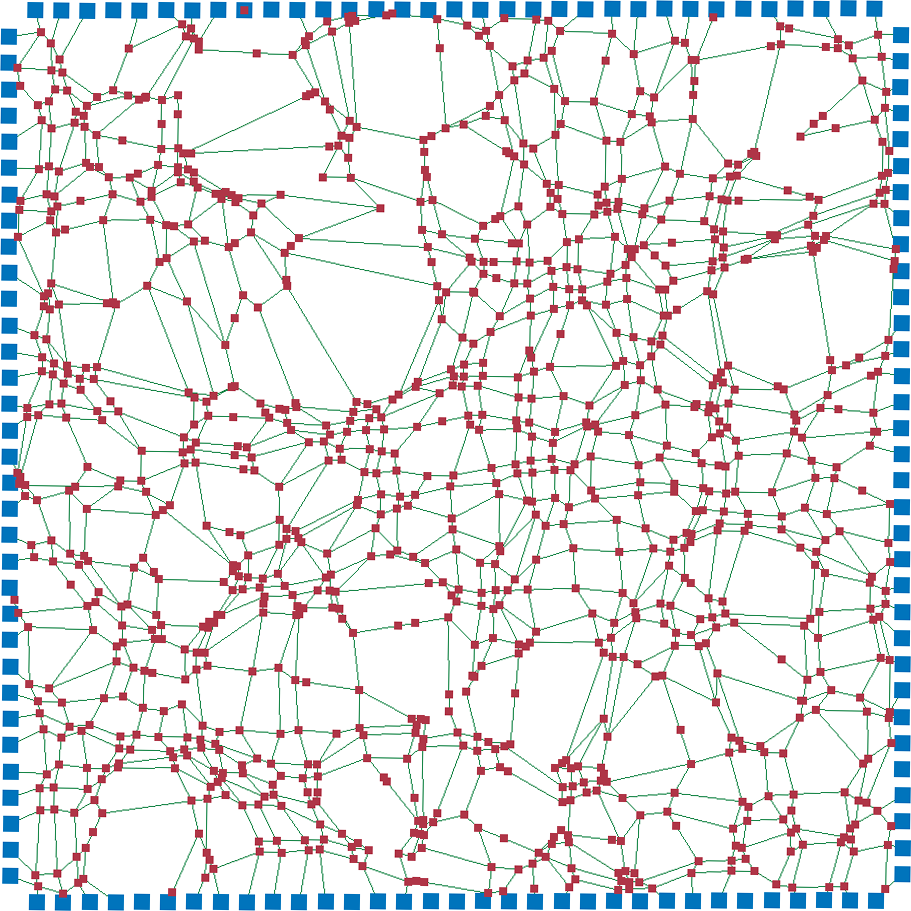
\includegraphics[
		width=\textwidth, 
		height=\textwidth, 
		keepaspectratio=true]
	{./img/results/1200_0_1_greater_104_step_3}
	\caption{}
	\label{fig:experiment:greaterThanStrain:3}
\end{subfigure}			

\begin{subfigure}{0.16\textwidth}
	\centering
	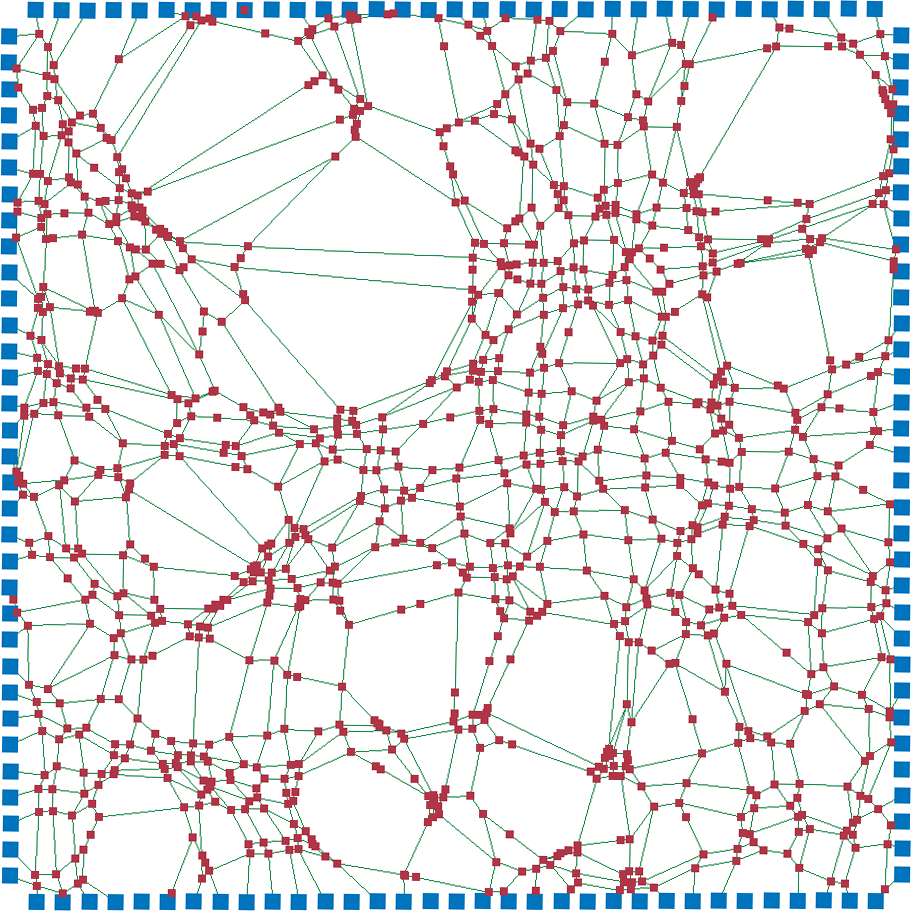
\includegraphics[
		width=\textwidth, 
		height=\textwidth, 
		keepaspectratio=true]
	{./img/results/1200_0_1_greater_104_step_4}
	\caption{}
	\label{fig:experiment:greaterThanStrain:4}
\end{subfigure}				
\begin{subfigure}{0.16\textwidth}
	\centering
	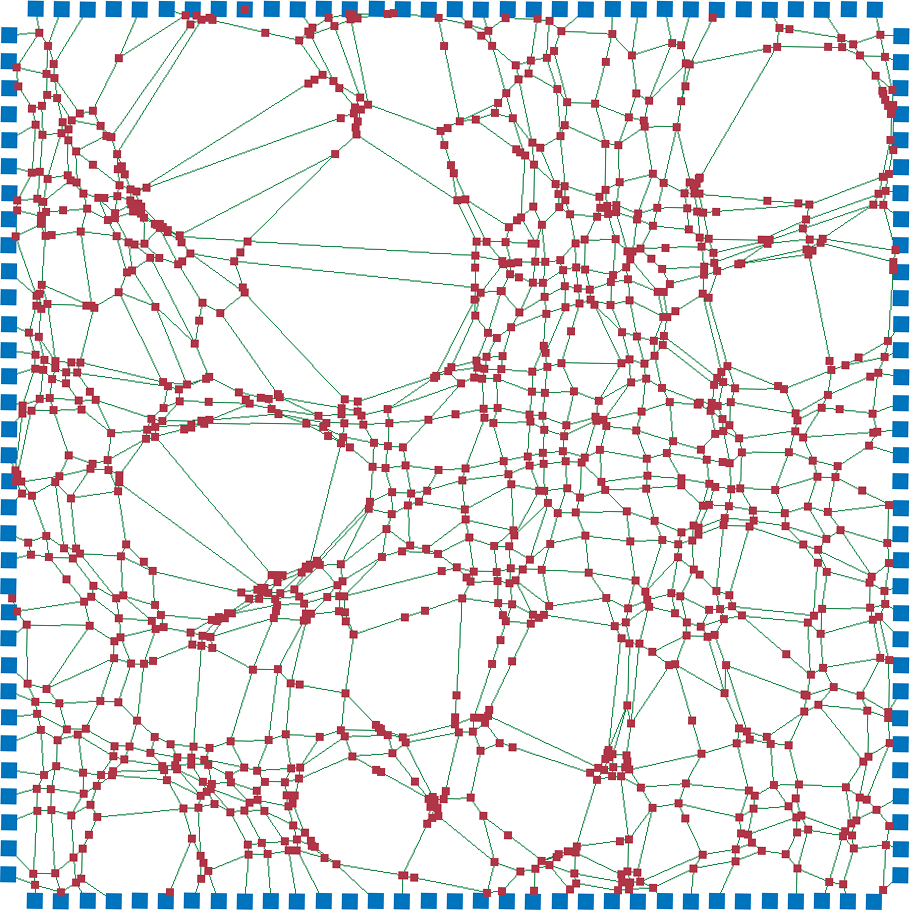
\includegraphics[
		width=\textwidth, 
		height=\textwidth, 
		keepaspectratio=true]
	{./img/results/1200_0_1_greater_104_step_5}
	\caption{}
	\label{fig:experiment:greaterThanStrain:5}
\end{subfigure}
\begin{subfigure}{0.16\textwidth}
	\centering
	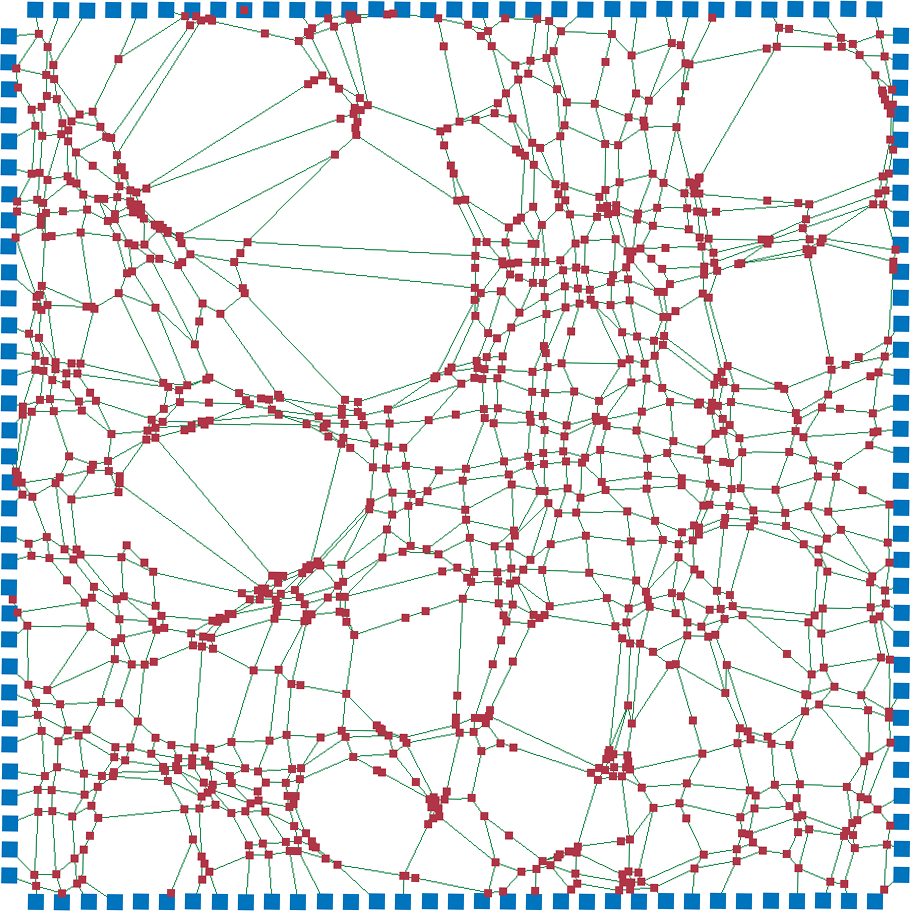
\includegraphics[
		width=\textwidth, 
		height=\textwidth, 
		keepaspectratio=true]
	{./img/results/1200_0_1_greater_104_step_6}
	\caption{}
	\label{fig:experiment:greaterThanStrain:6}
\end{subfigure}	
\begin{subfigure}{0.16\textwidth}
	\centering
	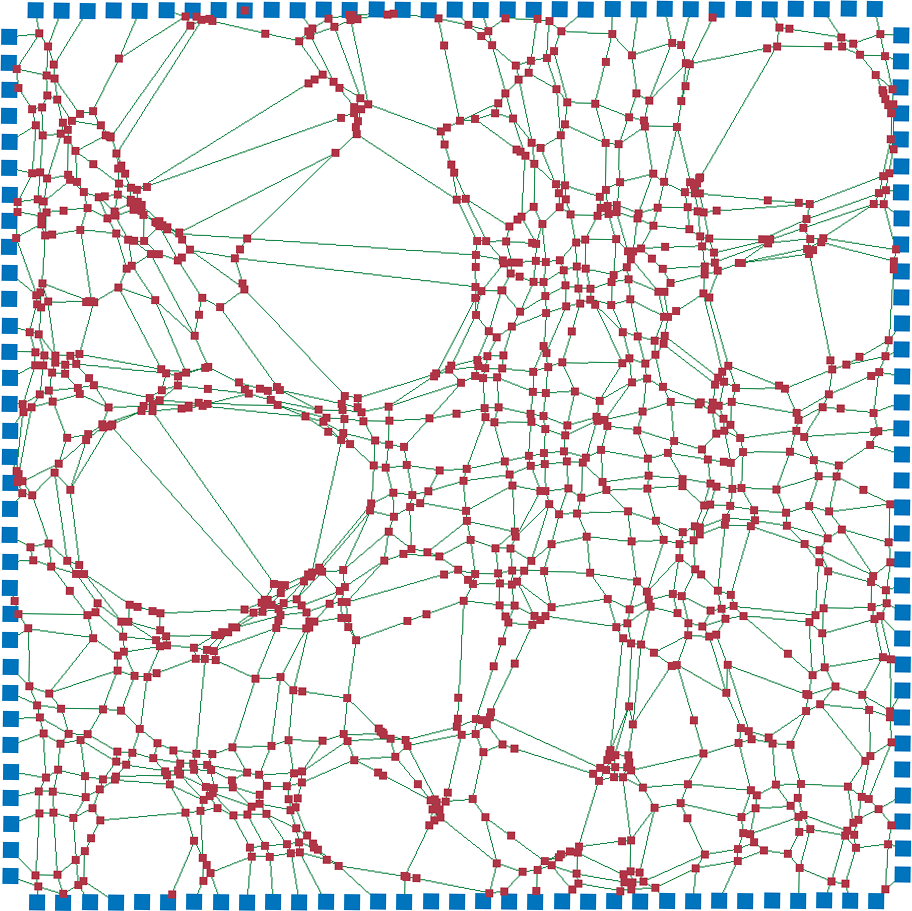
\includegraphics[
		width=\textwidth, 
		height=\textwidth, 
		keepaspectratio=true]
	{./img/results/1200_0_1_greater_104_step_7}
	\caption{}
	\label{fig:experiment:greaterThanStrain:7}
\end{subfigure}							
		\caption{Several steps of the simulation where at each step where springs are broken the springs with a strain greater than 1.04 are broken.}
		\label{fig:experiment:greaterThanStrain}
	\end{figure*}
	In \cref{fig:experiment:greaterThanStrain} steps of the simulation where springs are broken if there strain is greater then 1.04 are shown. Initially the results are comparable to those presented in \cref{fig:experiment:highestStrain}, however as the simulation progress the results are more like cracking mud, than a popping balloon. In \cref{fig:experiment:greaterThanStrain:7} there are no more springs to break, as the strain on any spring is smaller than $1.04$. Once could consider this state as a completely dried layer of matter, and adjust the threshold strain according to the material. Alternatively one could choose to decrease the strain threshold as the simulation advances.
	
% Stretch x with highest strain
	\begin{figure*}
		\centering
		%!TEX root = report.tex	
\begin{subfigure}{0.16\textwidth}
	\centering
	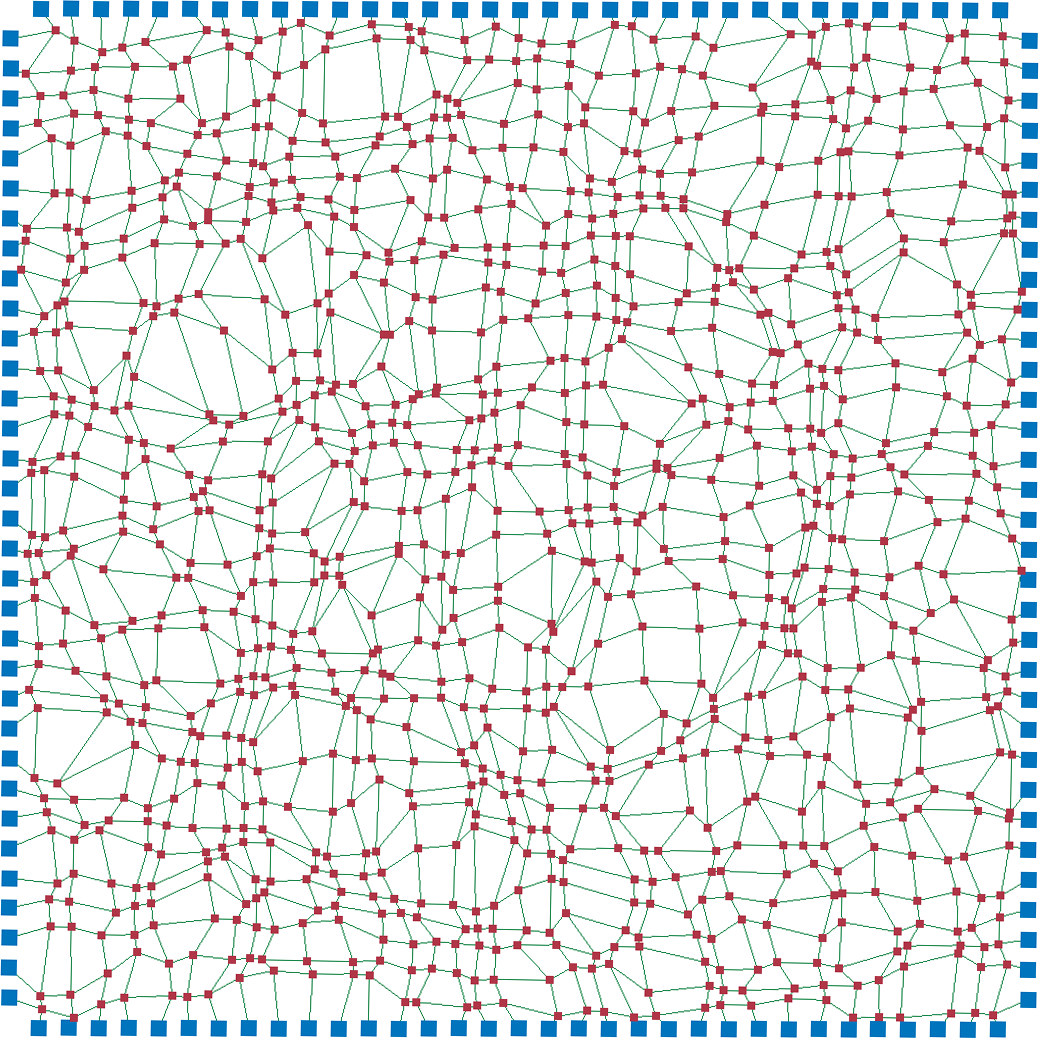
\includegraphics[
		width=\textwidth, 
		height=\textwidth, 
		keepaspectratio=true]
	{./img/results/1200_0_1_stretchGreaterThan_104_step_1}
	%\caption{Step 0}
	%\label{fig:experiment:stretchGreaterThanStrain:1}
\end{subfigure}	
\begin{subfigure}{0.16\textwidth}
	\centering
	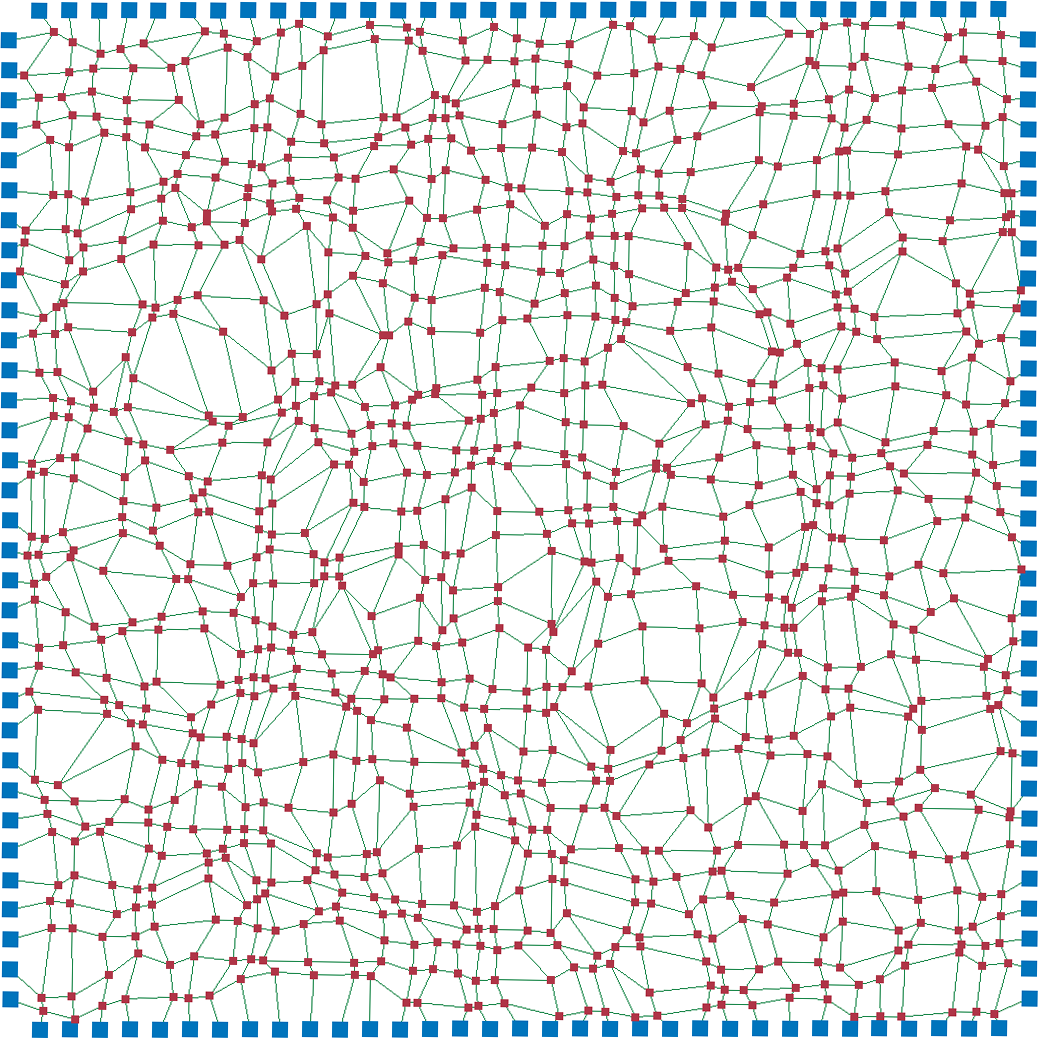
\includegraphics[
		width=\textwidth, 
		height=\textwidth, 
		keepaspectratio=true]
	{./img/results/1200_0_1_stretchGreaterThan_104_step_2}
	%\caption{Step 1}
	%\label{fig:experiment:stretchGreaterThanStrain:2}
\end{subfigure}		
\begin{subfigure}{0.16\textwidth}
	\centering
	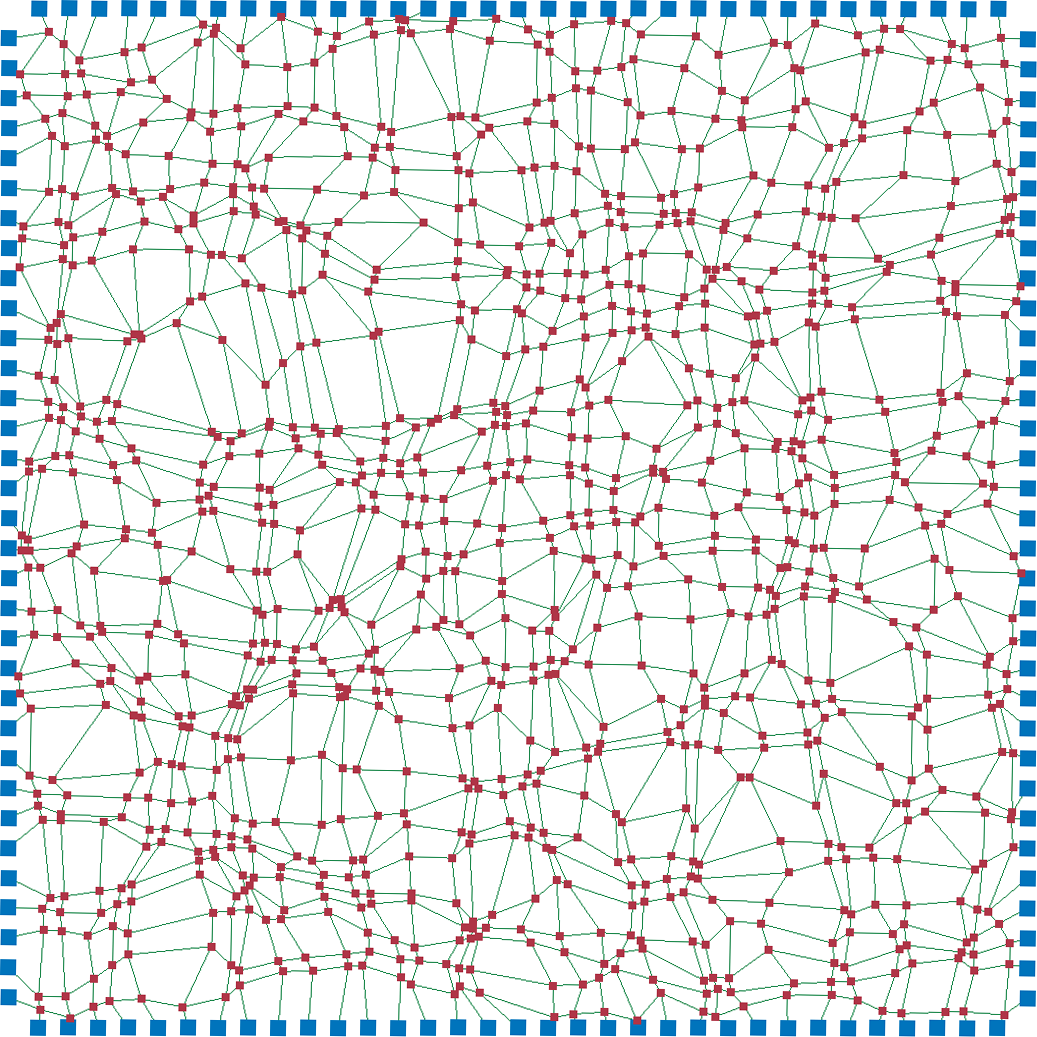
\includegraphics[
		width=\textwidth, 
		height=\textwidth, 
		keepaspectratio=true]
	{./img/results/1200_0_1_stretchGreaterThan_104_step_3}
	%\caption{Step 2}
	%\label{fig:experiment:stretchGreaterThanStrain:3}
\end{subfigure}			
\begin{subfigure}{0.16\textwidth}
	\centering
	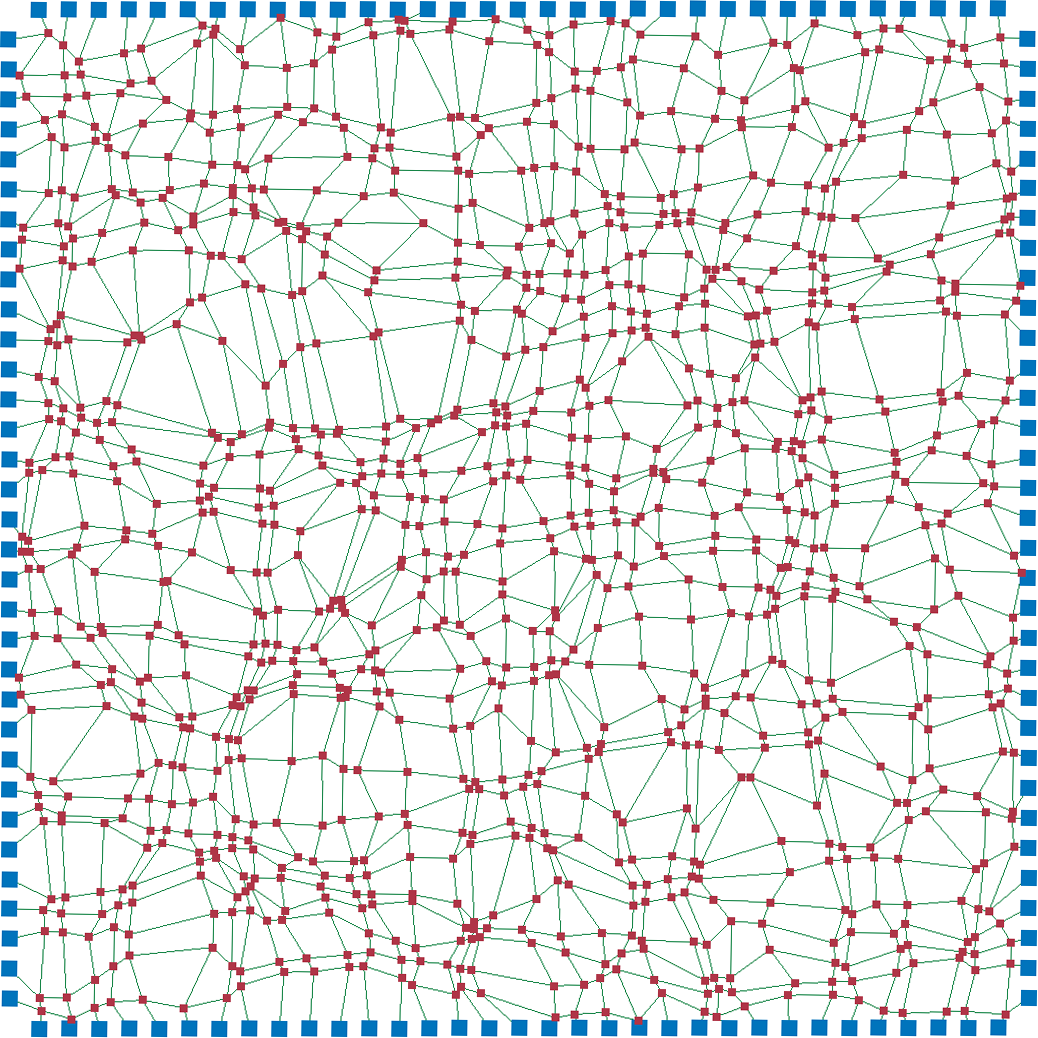
\includegraphics[
		width=\textwidth, 
		height=\textwidth, 
		keepaspectratio=true]
	{./img/results/1200_0_1_stretchGreaterThan_104_step_4}
	%\caption{Step 3}
	%\label{fig:experiment:stretchGreaterThanStrain:4}
\end{subfigure}				
\begin{subfigure}{0.16\textwidth}
	\centering
	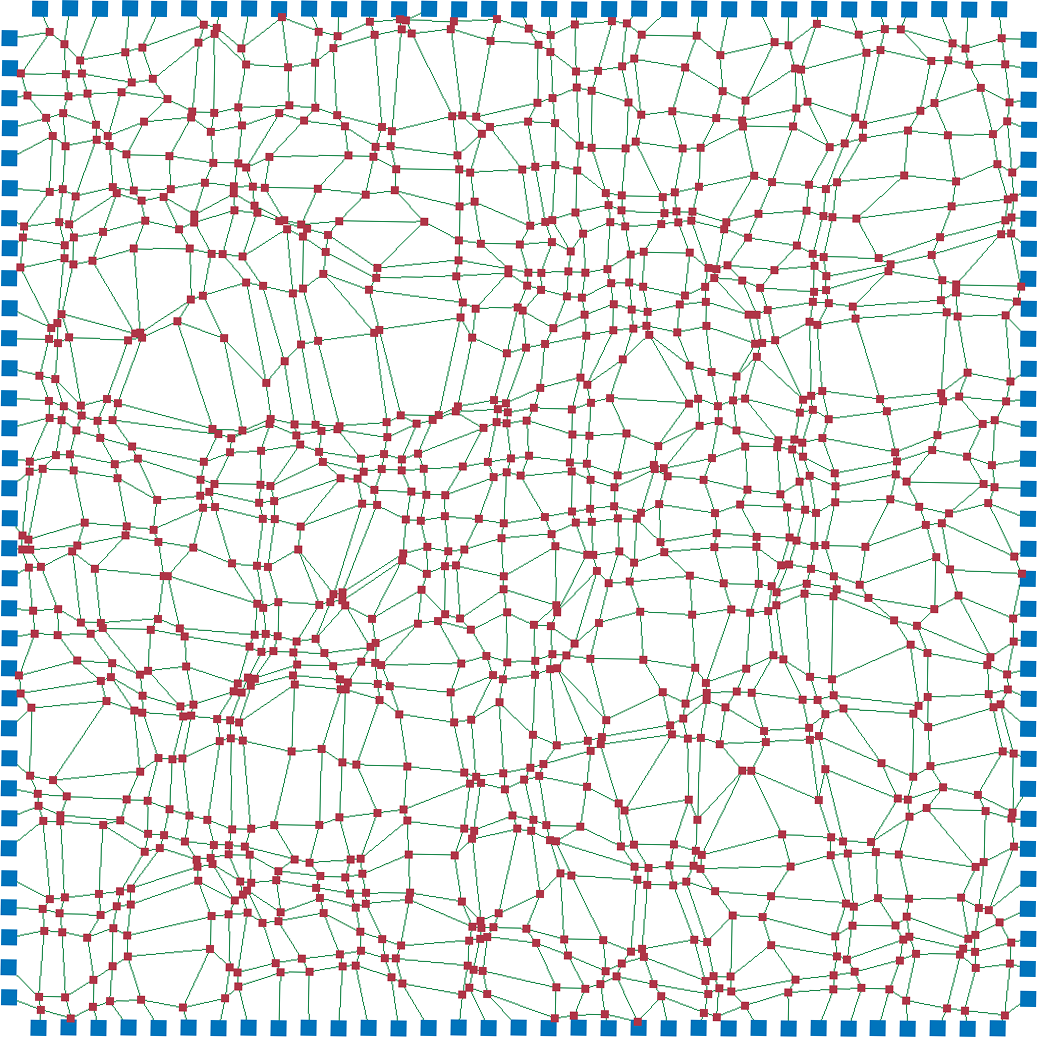
\includegraphics[
		width=\textwidth, 
		height=\textwidth, 
		keepaspectratio=true]
	{./img/results/1200_0_1_stretchGreaterThan_104_step_5}
	%\caption{Step 4}
	%\label{fig:experiment:stretchGreaterThanStrain:5}
\end{subfigure}					
		\caption{Several steps of the simulation where at each step where springs are stretch the 97 springs with the highest strain are stretched.}
		\label{fig:experiment:stretchGreaterThanStrain}
	\end{figure*}
	\todo[inline]{Discuss results of stretching springs with highest strain.}

% Stretch x with strain >
	\begin{figure*}
		\centering
		%!TEX root = report.tex	
\begin{subfigure}{0.16\textwidth}
	\centering
	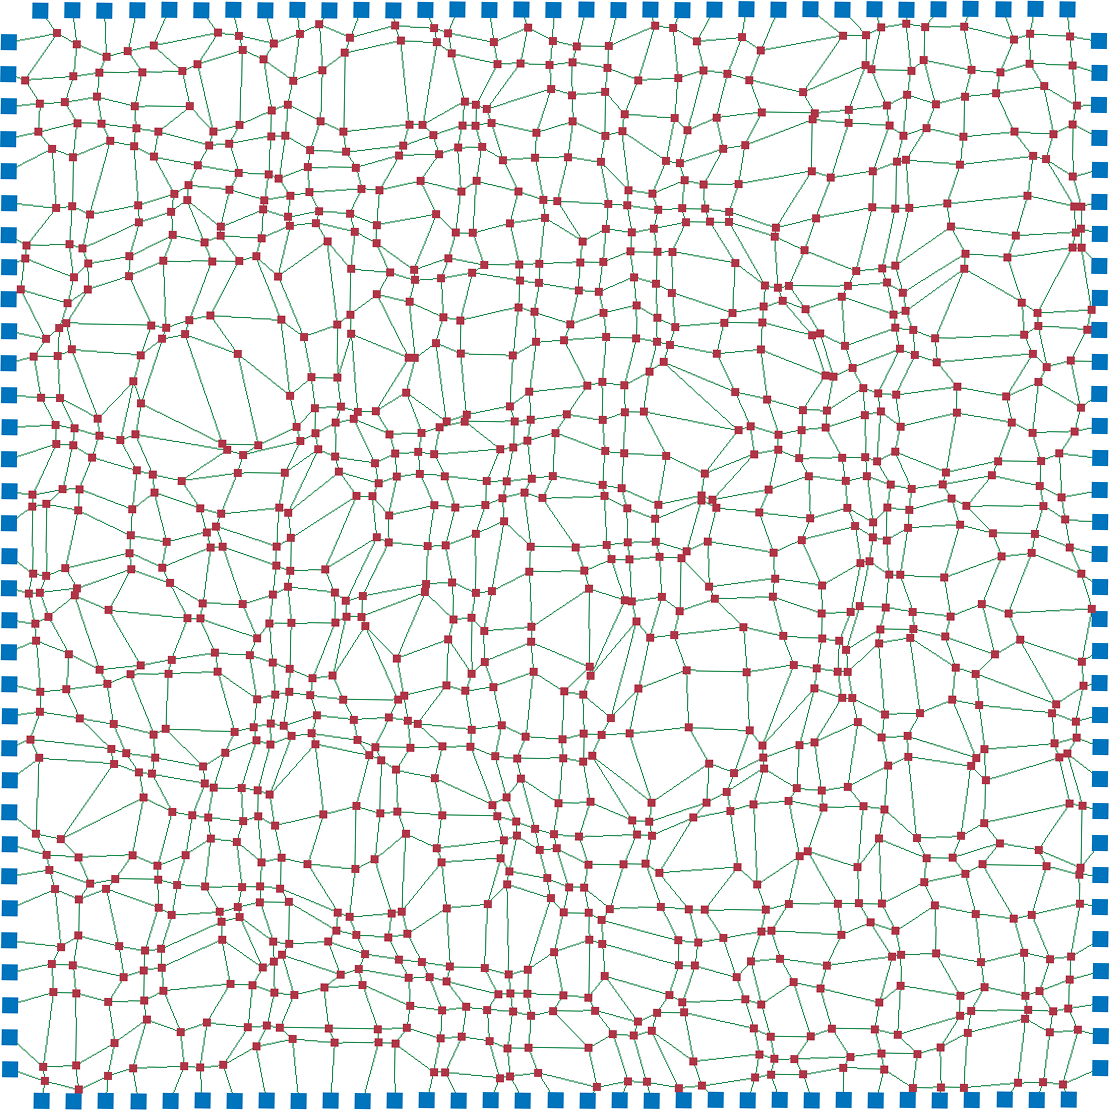
\includegraphics[
		width=\textwidth, 
		height=\textwidth, 
		keepaspectratio=true]
	{./img/results/1200_0_1_stretchHighest_97_step_0}
	\caption{Step 0}
	\label{fig:experiment:stretchHighestStrain:0}
\end{subfigure}	
\begin{subfigure}{0.16\textwidth}
	\centering
	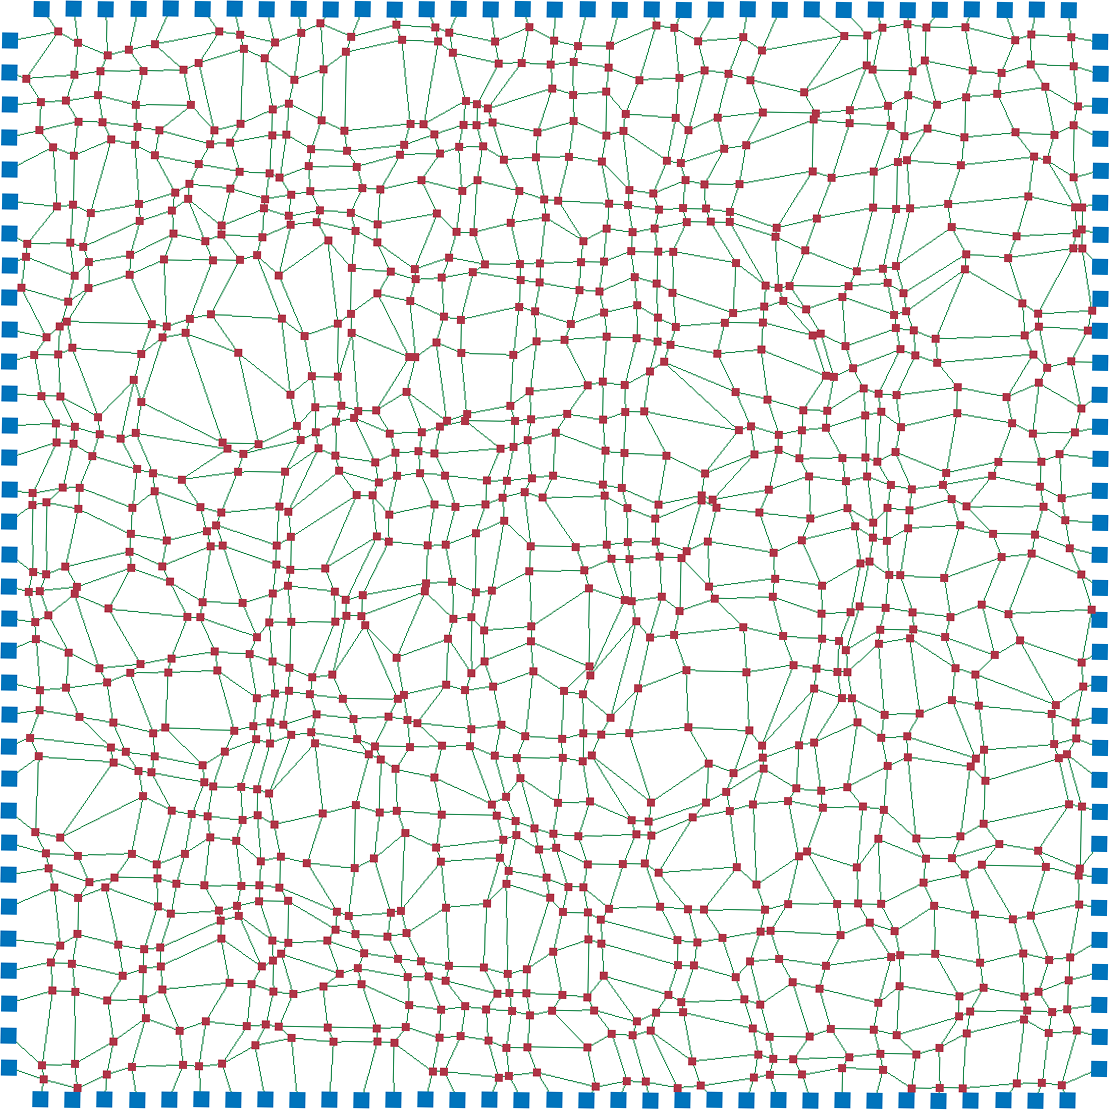
\includegraphics[
		width=\textwidth, 
		height=\textwidth, 
		keepaspectratio=true]
	{./img/results/1200_0_1_stretchHighest_97_step_1}
	\caption{Step 1}
	\label{fig:experiment:stretchHighestStrain:1}
\end{subfigure}		
\begin{subfigure}{0.16\textwidth}
	\centering
	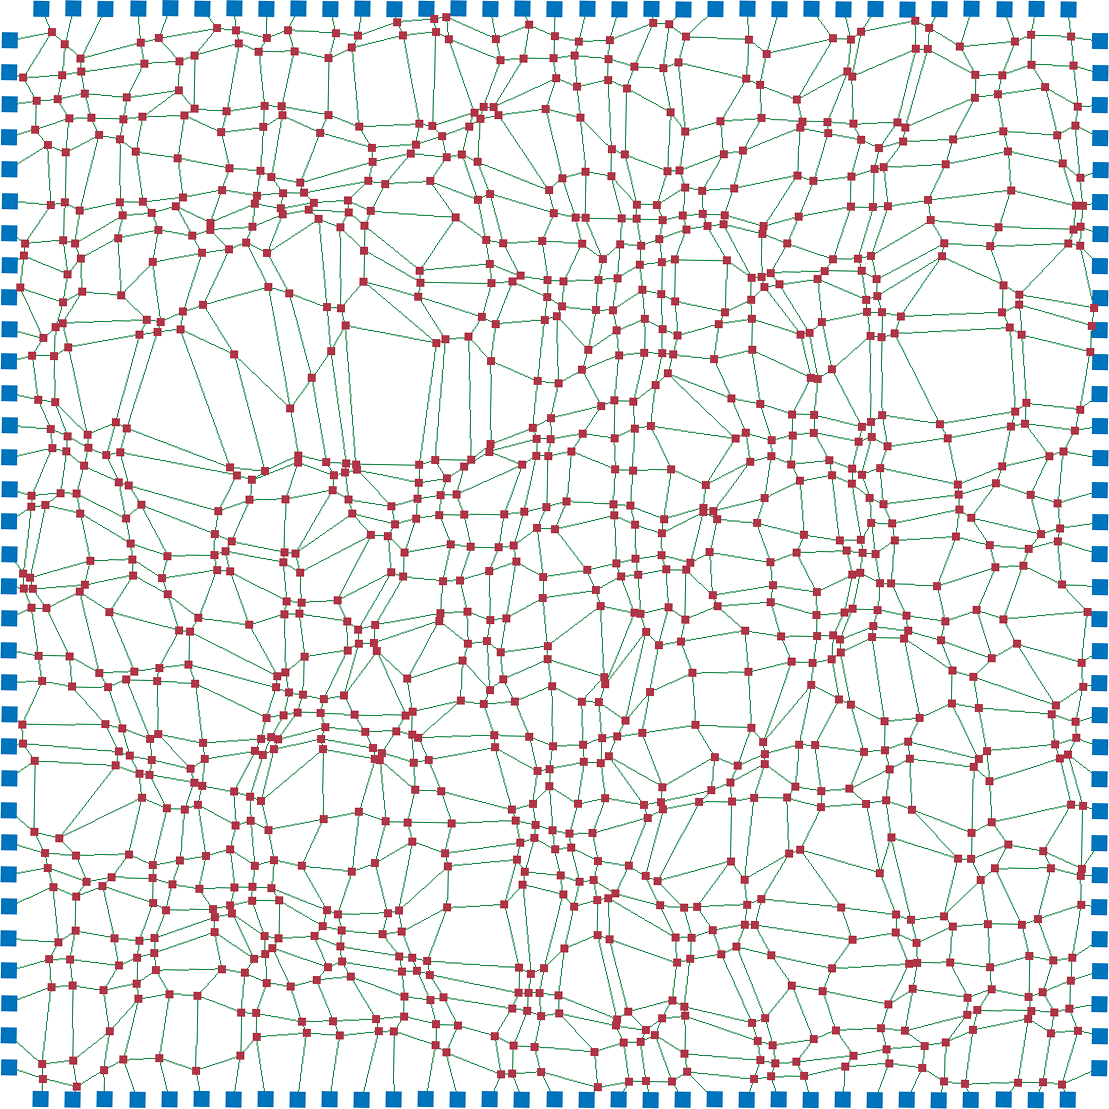
\includegraphics[
		width=\textwidth, 
		height=\textwidth, 
		keepaspectratio=true]
	{./img/results/1200_0_1_stretchHighest_97_step_2}
	\caption{Step 2}
	\label{fig:experiment:stretchHighestStrain:2}
\end{subfigure}			
\begin{subfigure}{0.16\textwidth}
	\centering
	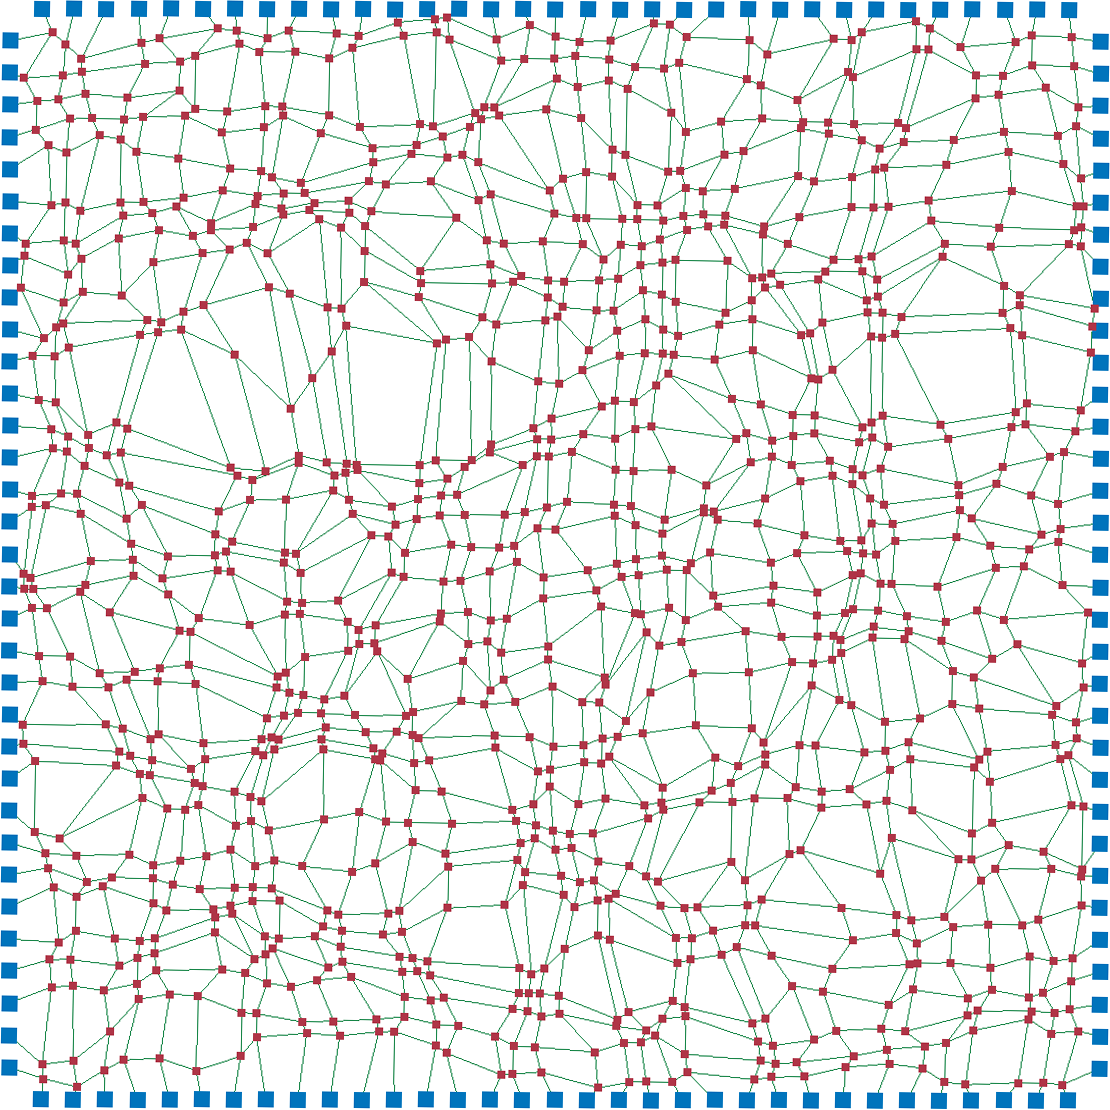
\includegraphics[
		width=\textwidth, 
		height=\textwidth, 
		keepaspectratio=true]
	{./img/results/1200_0_1_stretchHighest_97_step_3}
	\caption{Step 3}
	\label{fig:experiment:stretchHighestStrain:3}
\end{subfigure}				
\begin{subfigure}{0.16\textwidth}
	\centering
	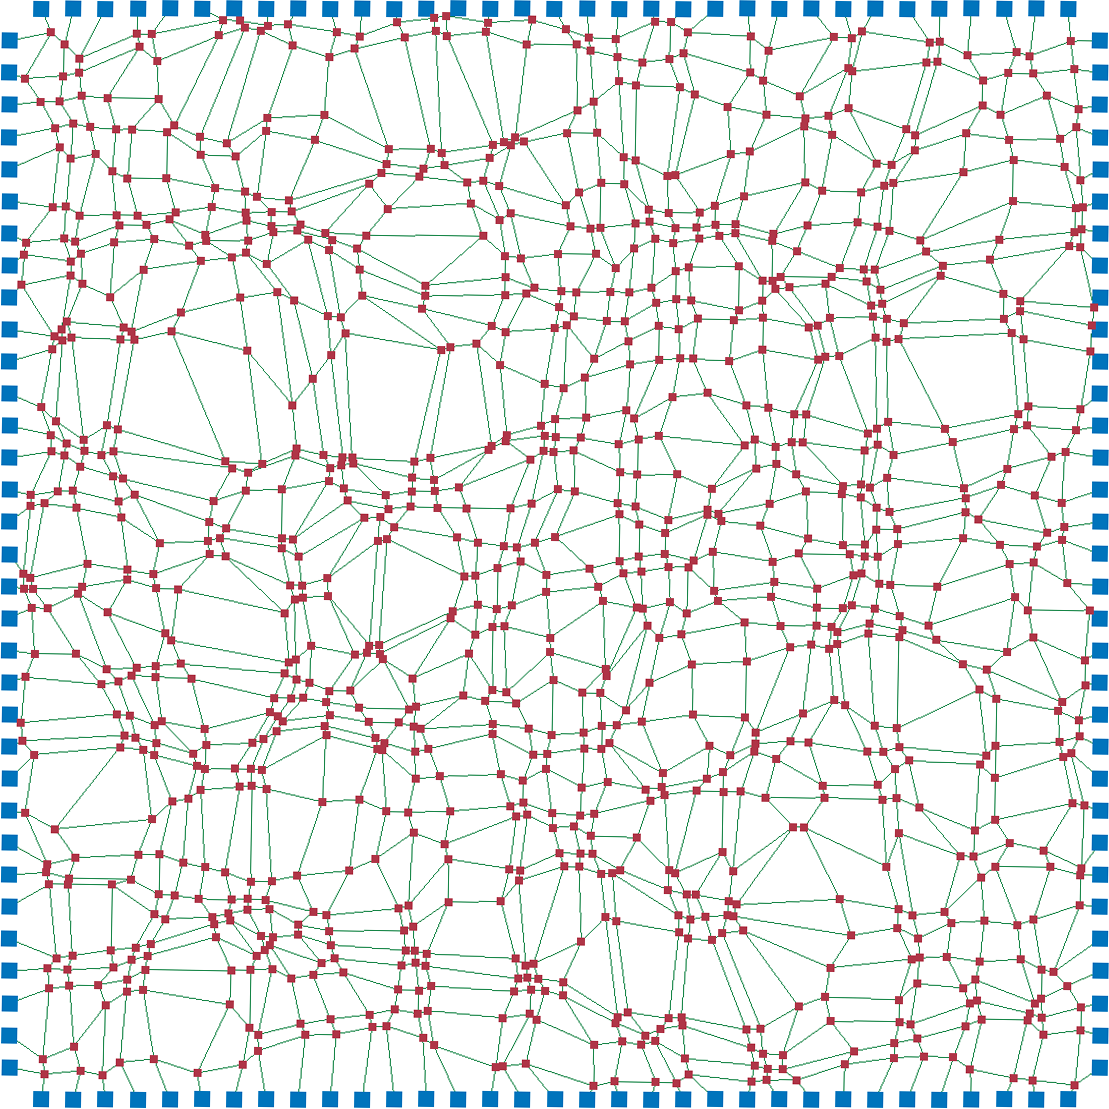
\includegraphics[
		width=\textwidth, 
		height=\textwidth, 
		keepaspectratio=true]
	{./img/results/1200_0_1_stretchHighest_97_step_4}
	\caption{Step 4}
	\label{fig:experiment:stretchHighestStrain:4}
\end{subfigure}
\begin{subfigure}{0.16\textwidth}
	\centering
	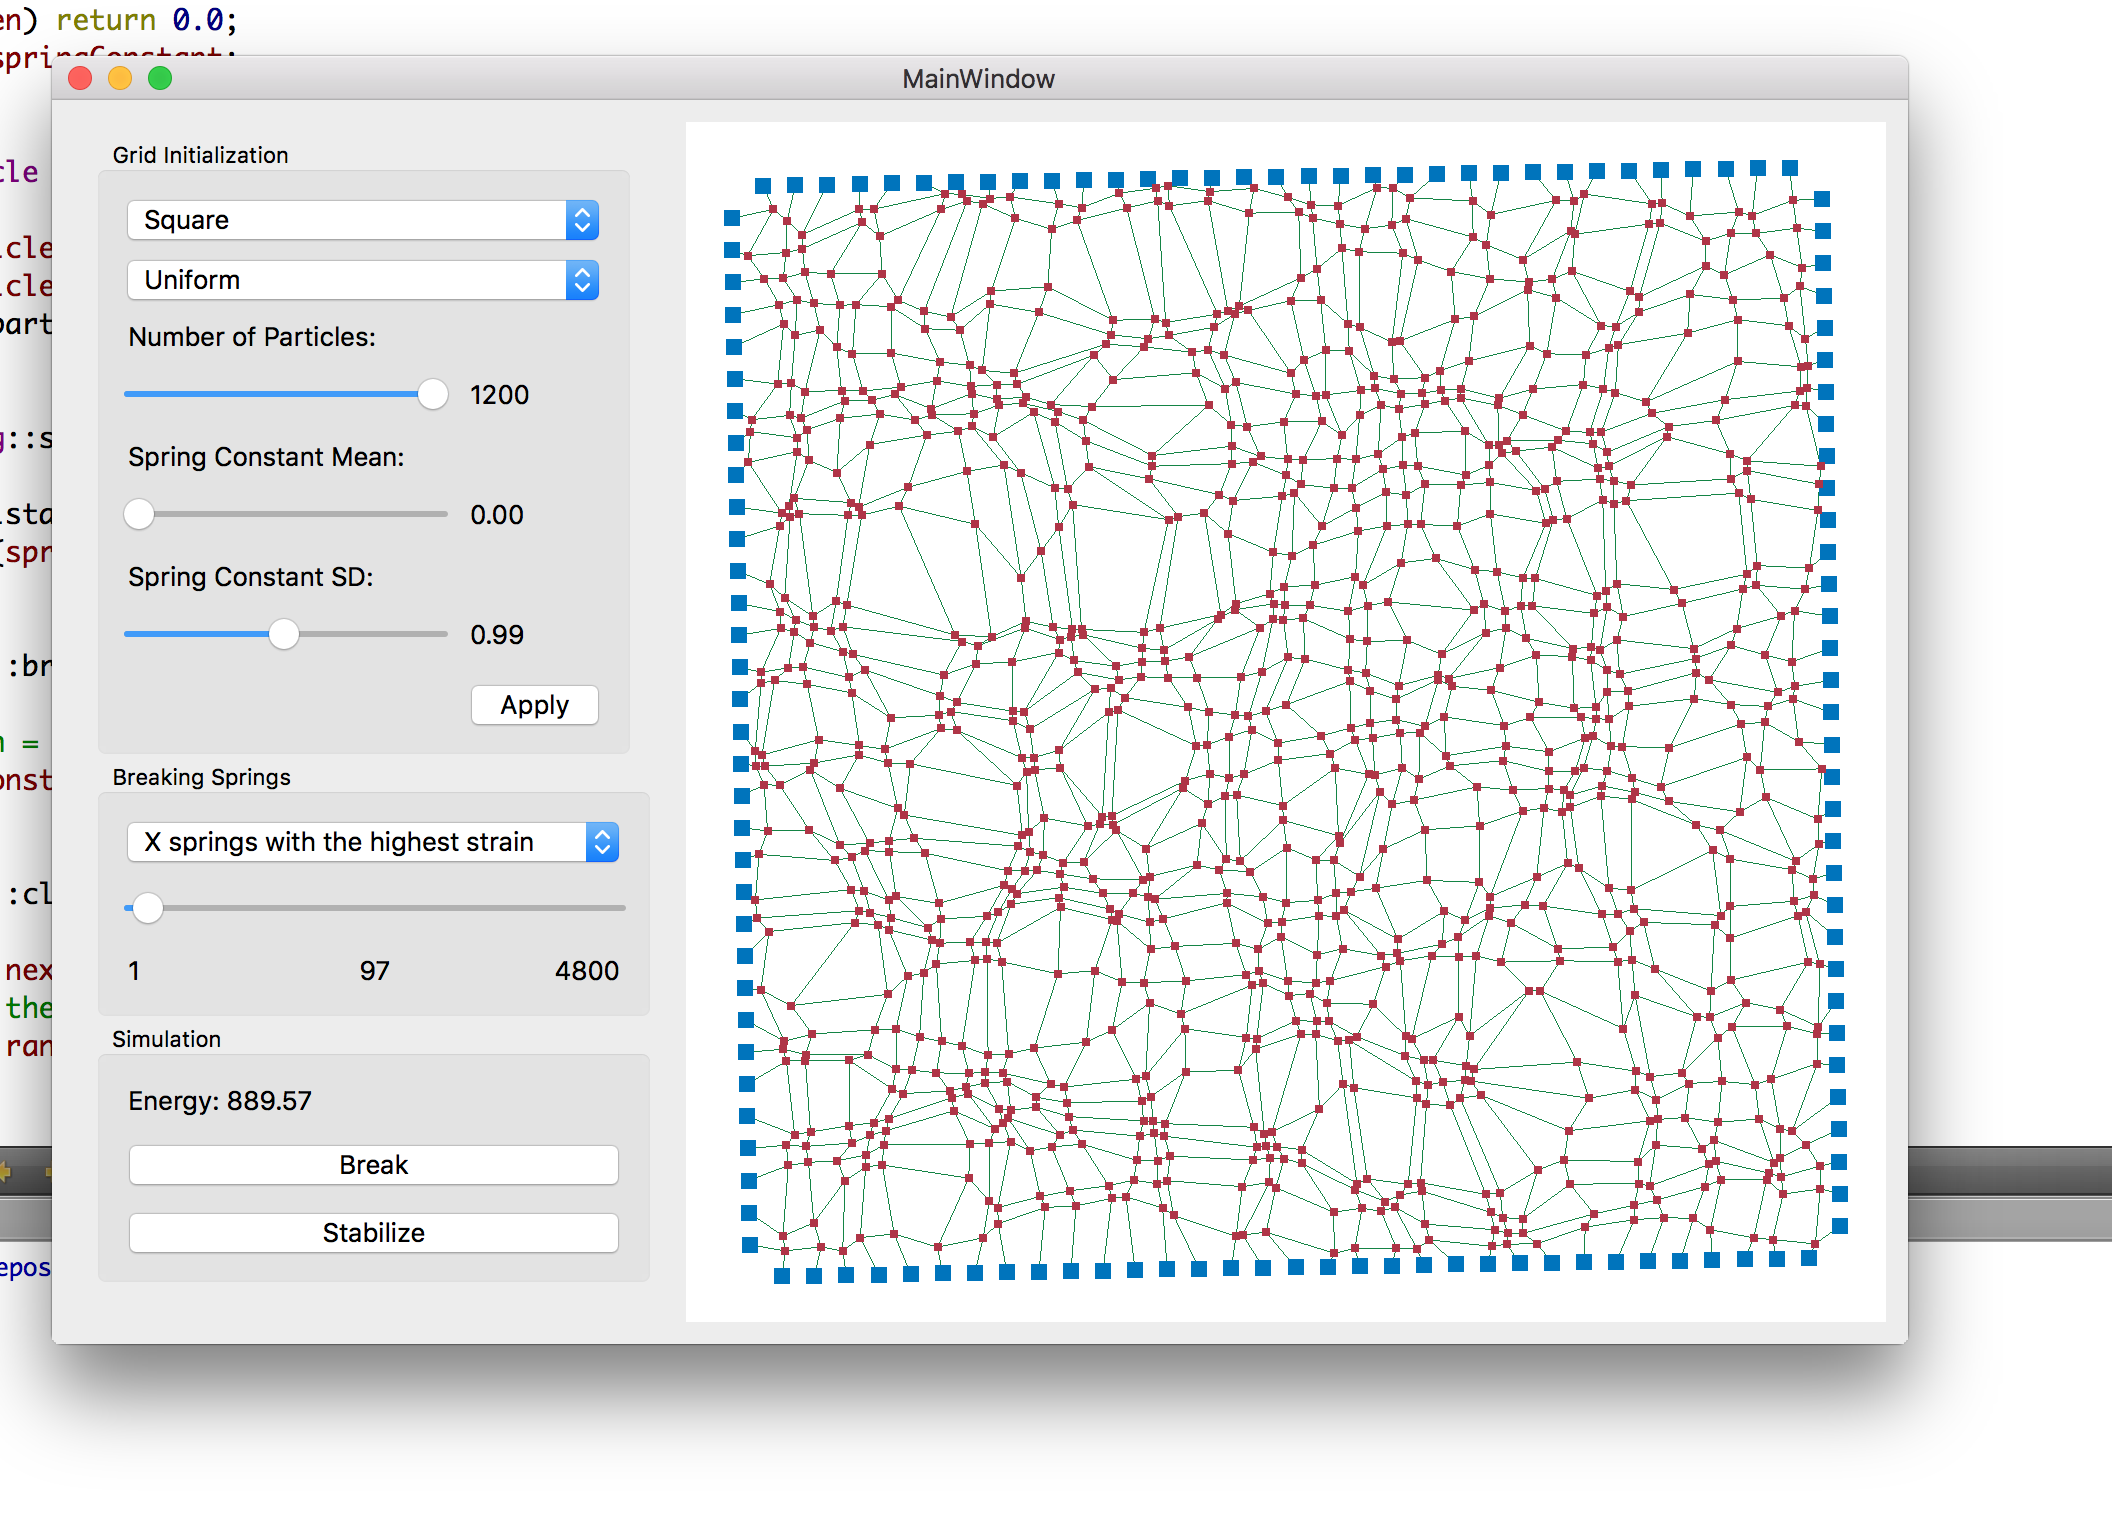
\includegraphics[
		width=\textwidth, 
		height=\textwidth, 
		keepaspectratio=true]
	{./img/results/1200_0_1_stretchHighest_97_step_5}
	\caption{Step 4}
	\label{fig:experiment:stretchHighestStrain:5}
\end{subfigure}

\begin{subfigure}{0.16\textwidth}
	\centering
	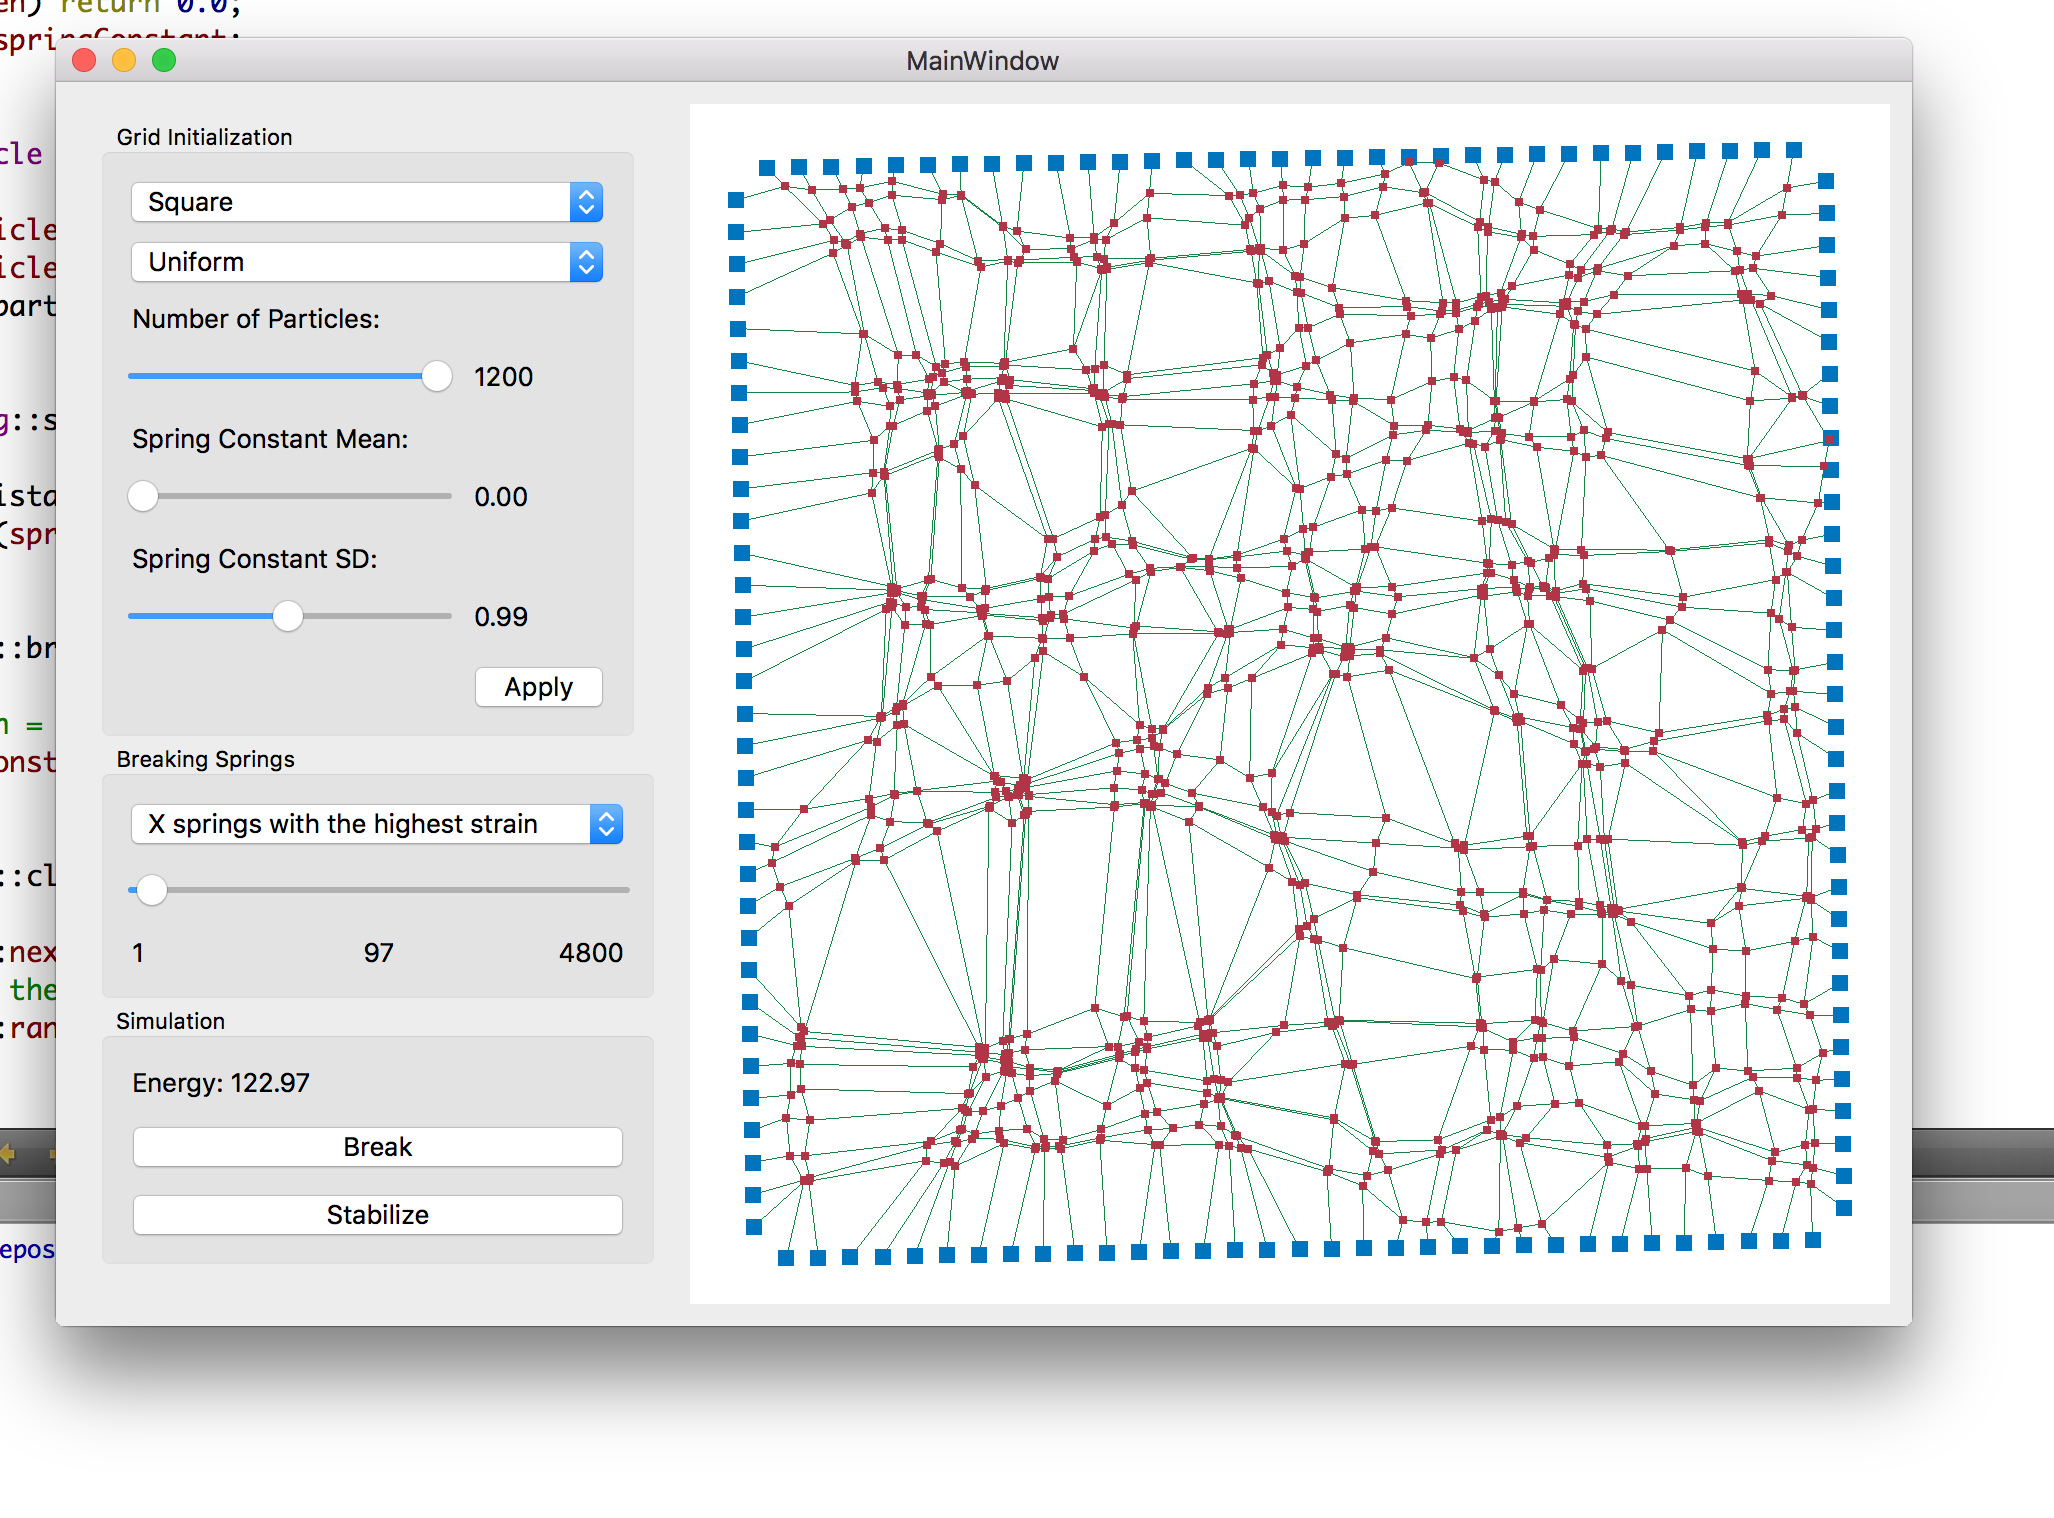
\includegraphics[
		width=\textwidth, 
		height=\textwidth, 
		keepaspectratio=true]
	{./img/results/1200_0_1_stretchHighest_97_step_50}
	\caption{Step 50}
	\label{fig:expe riment:stretchHighestStrain:50}
\end{subfigure}	
\begin{subfigure}{0.16\textwidth}
	\centering
	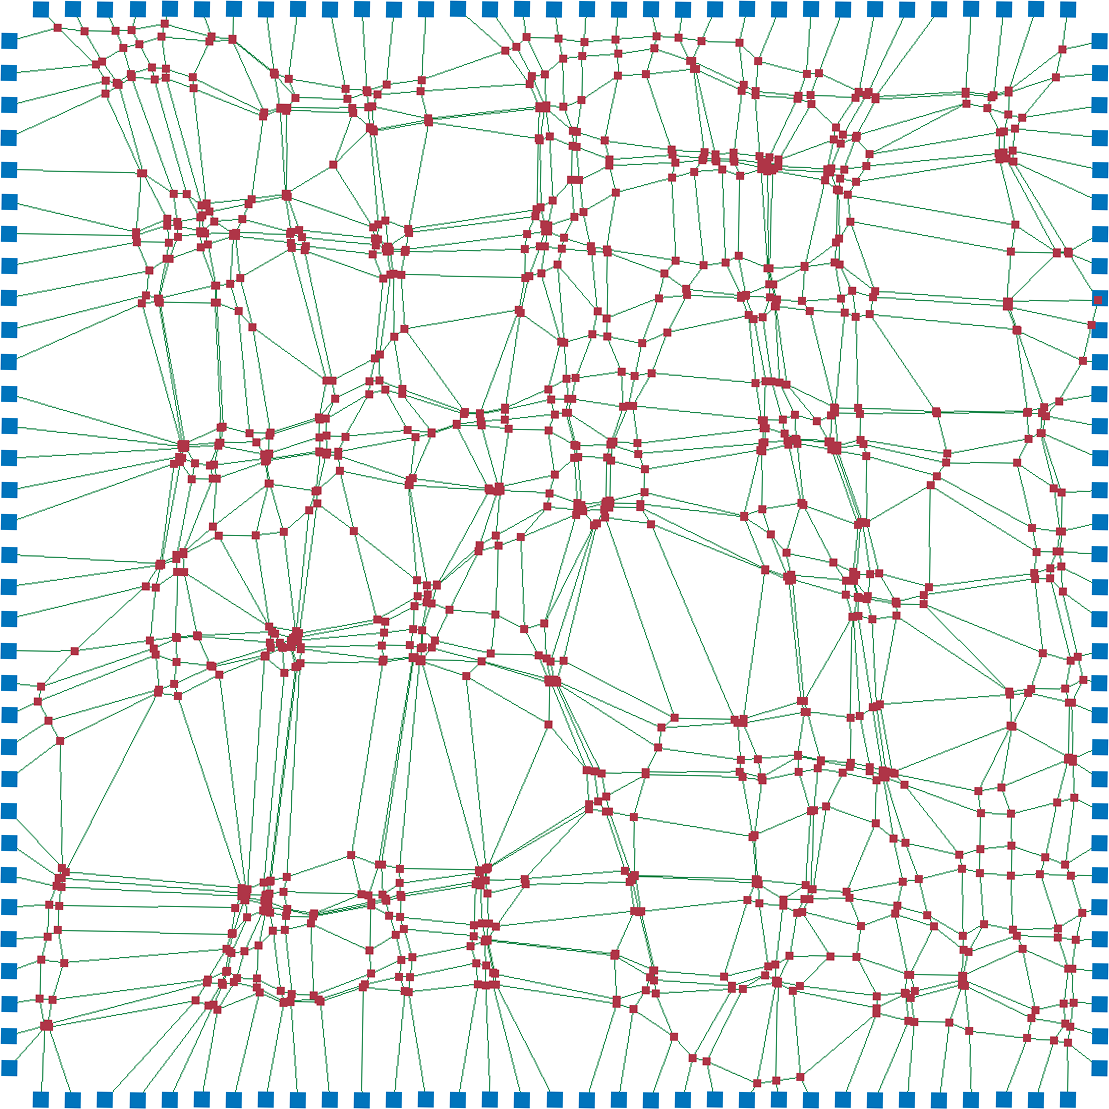
\includegraphics[
		width=\textwidth, 
		height=\textwidth, 
		keepaspectratio=true]
	{./img/results/1200_0_1_stretchHighest_97_step_51}
	\caption{Step 51}
	\label{fig:experiment:stretchHighestStrain:51}
\end{subfigure}		
\begin{subfigure}{0.16\textwidth}
	\centering
	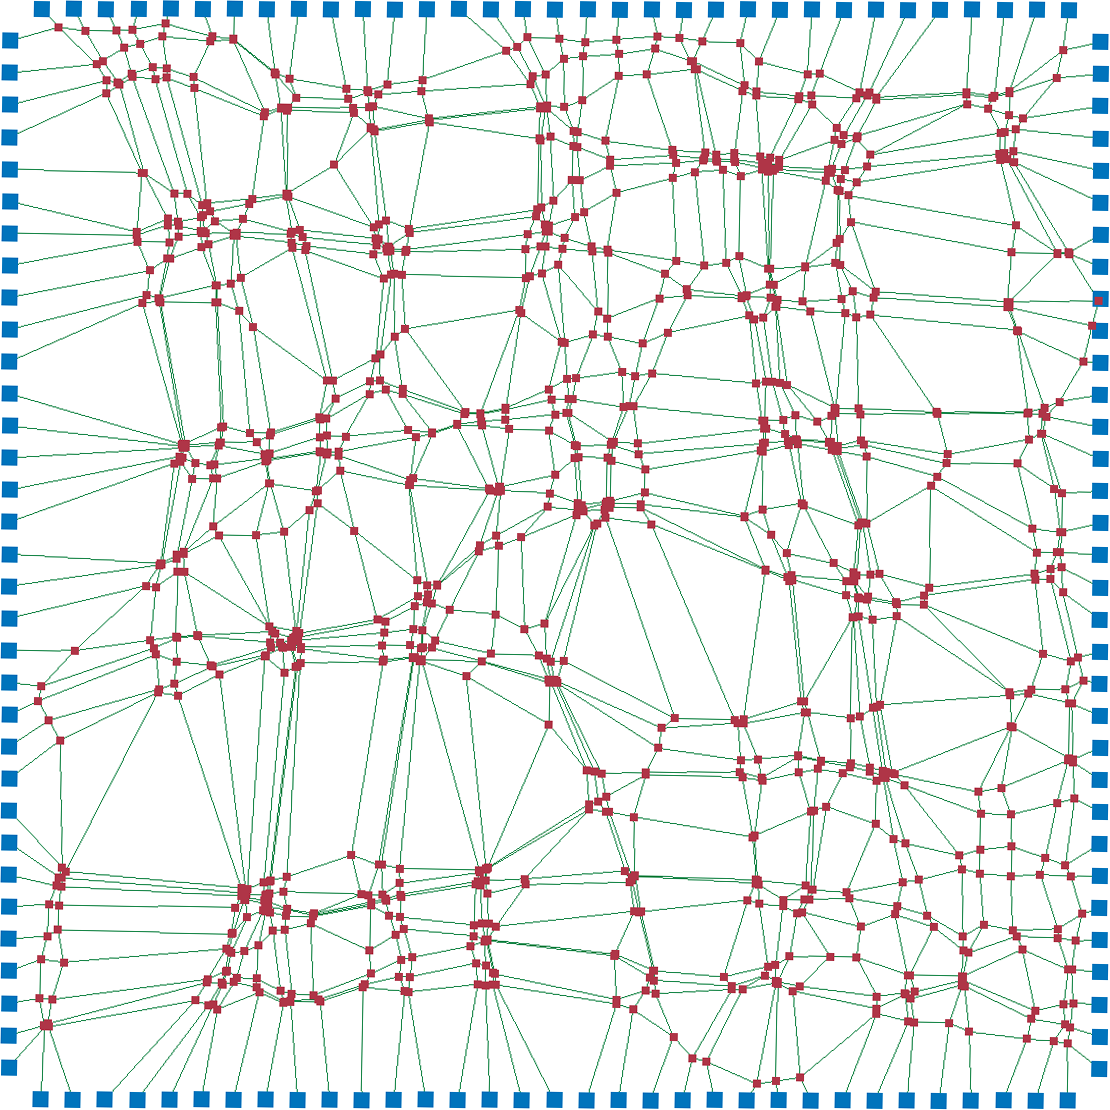
\includegraphics[
		width=\textwidth, 
		height=\textwidth, 
		keepaspectratio=true]
	{./img/results/1200_0_1_stretchHighest_97_step_52}
	\caption{Step 52}
	\label{fig:experiment:stretchHighestStrain:52}
\end{subfigure}			
\begin{subfigure}{0.16\textwidth}
	\centering
	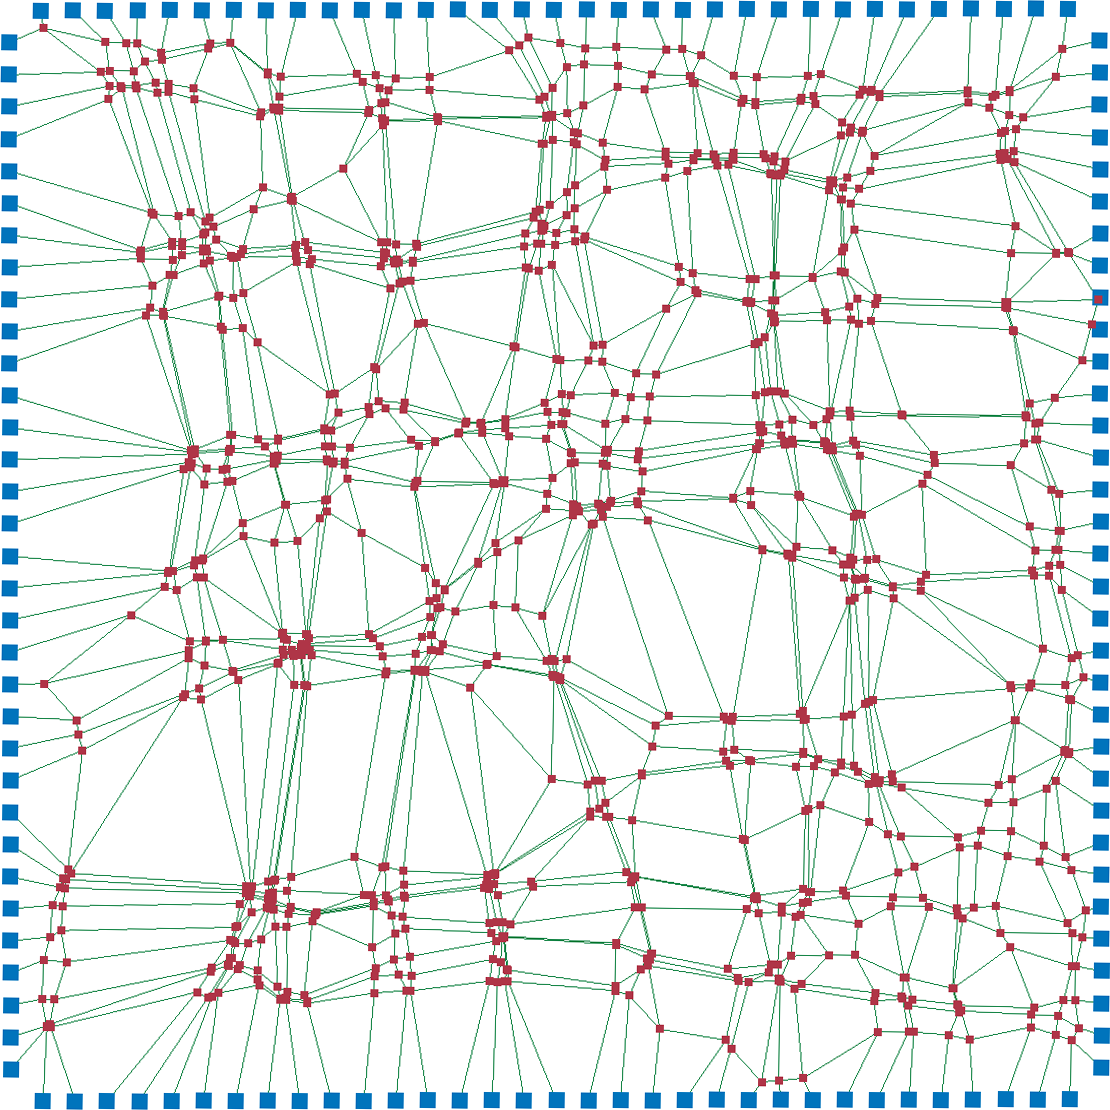
\includegraphics[
		width=\textwidth, 
		height=\textwidth, 
		keepaspectratio=true]
	{./img/results/1200_0_1_stretchHighest_97_step_53}
	\caption{Step 53}
	\label{fig:experiment:stretchHighestStrain:53}
\end{subfigure}				
\begin{subfigure}{0.16\textwidth}
	\centering
	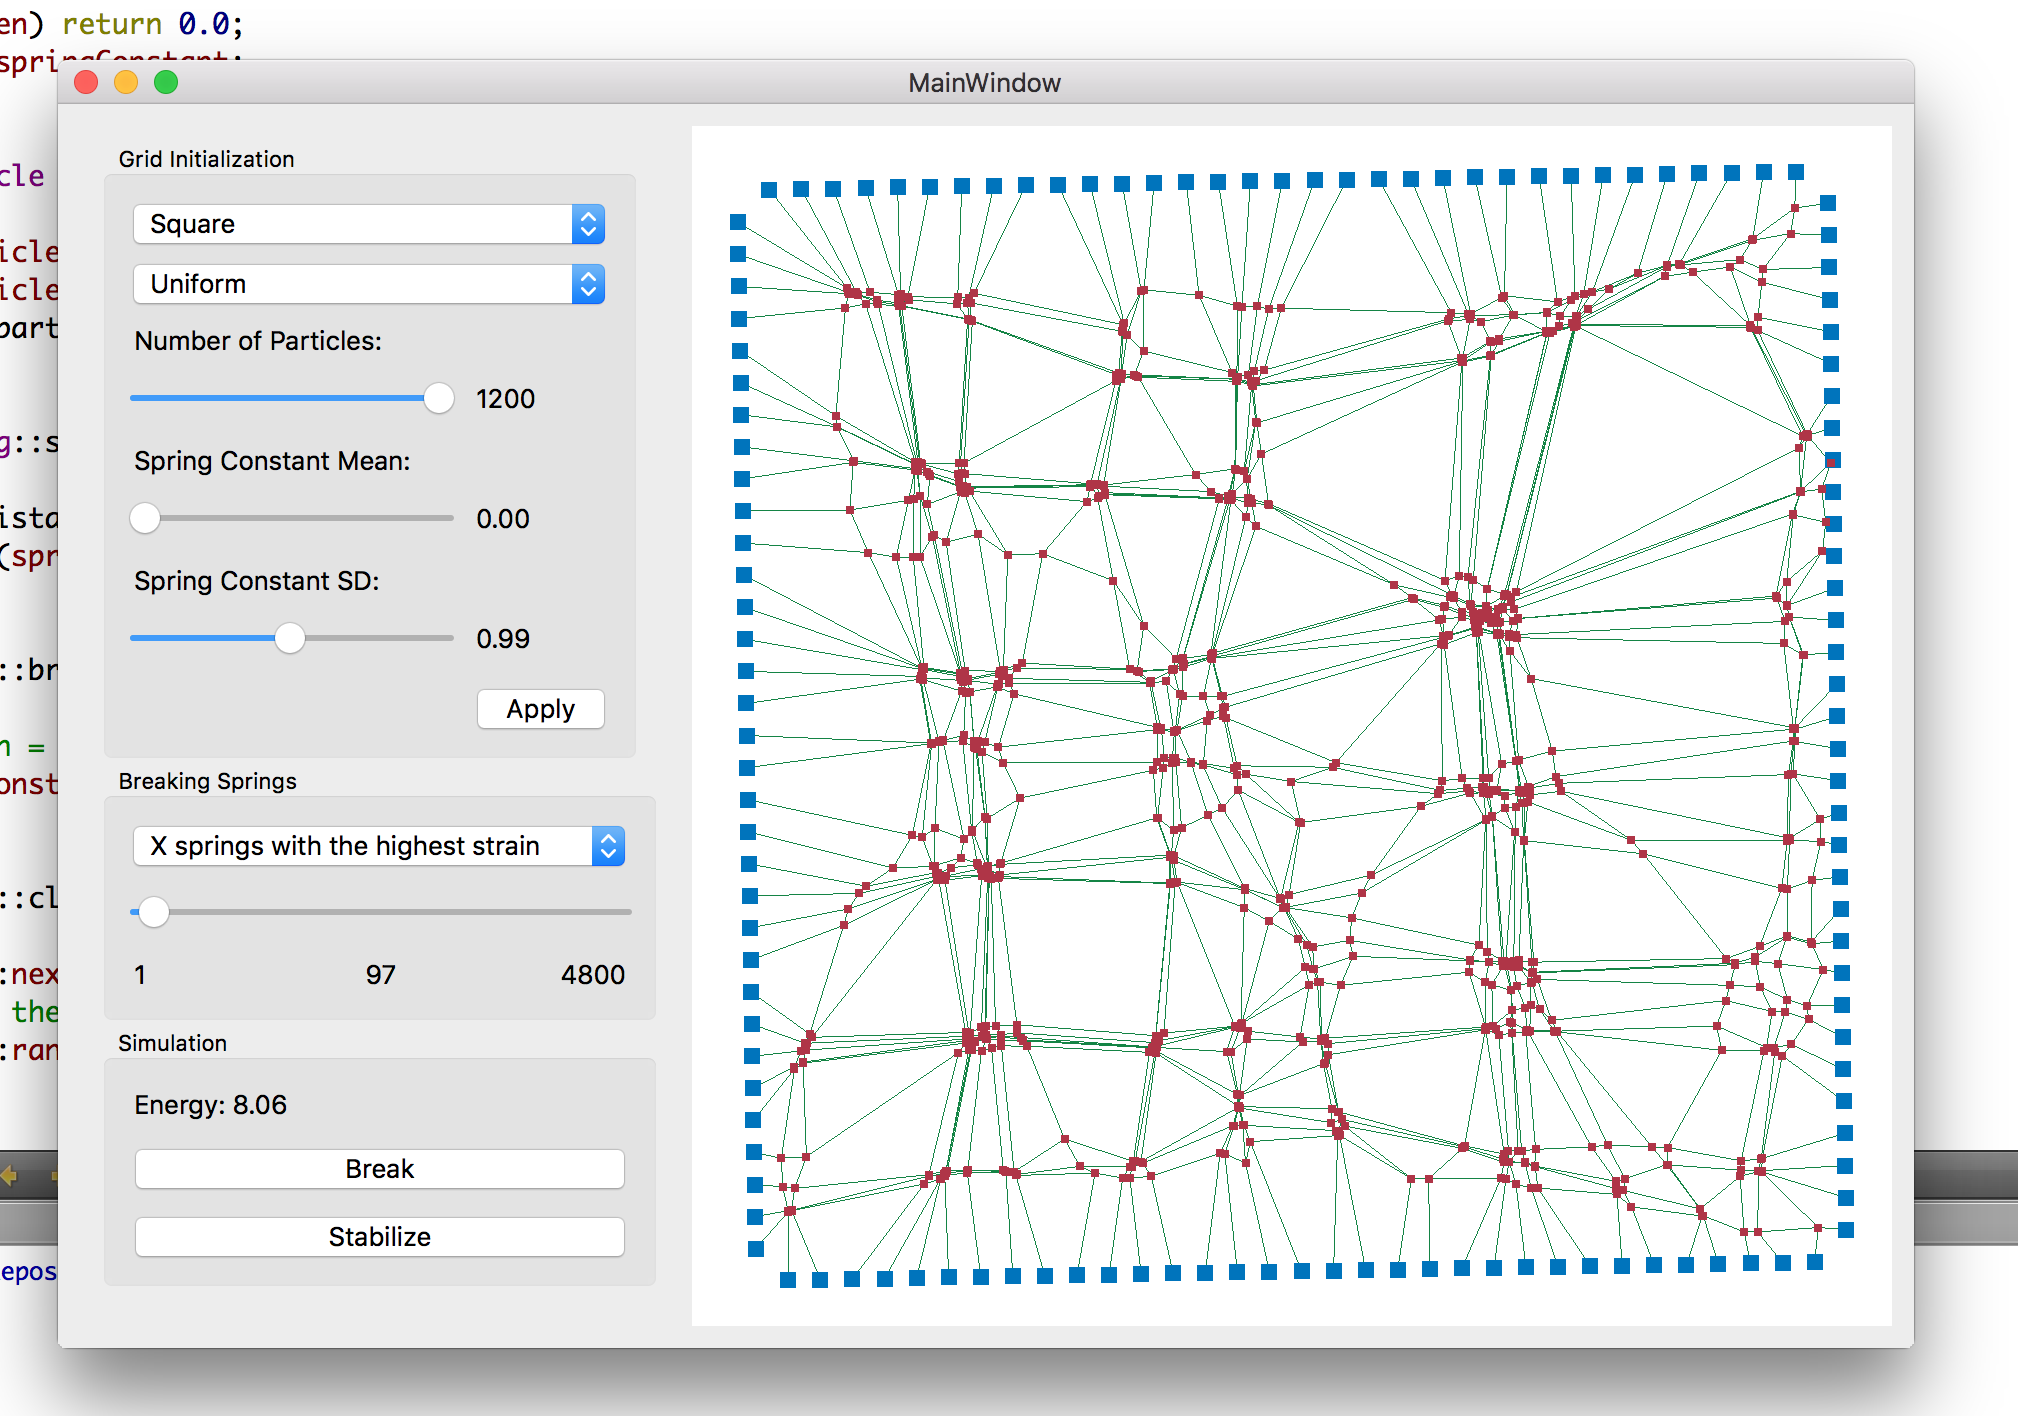
\includegraphics[
		width=\textwidth, 
		height=\textwidth, 
		keepaspectratio=true]
	{./img/results/1200_0_1_stretchHighest_97_step_80}
	\caption{Step 80}
	\label{fig:experiment:stretchHighestStrain:80}
\end{subfigure}
\begin{subfigure}{0.16\textwidth}
	\centering
	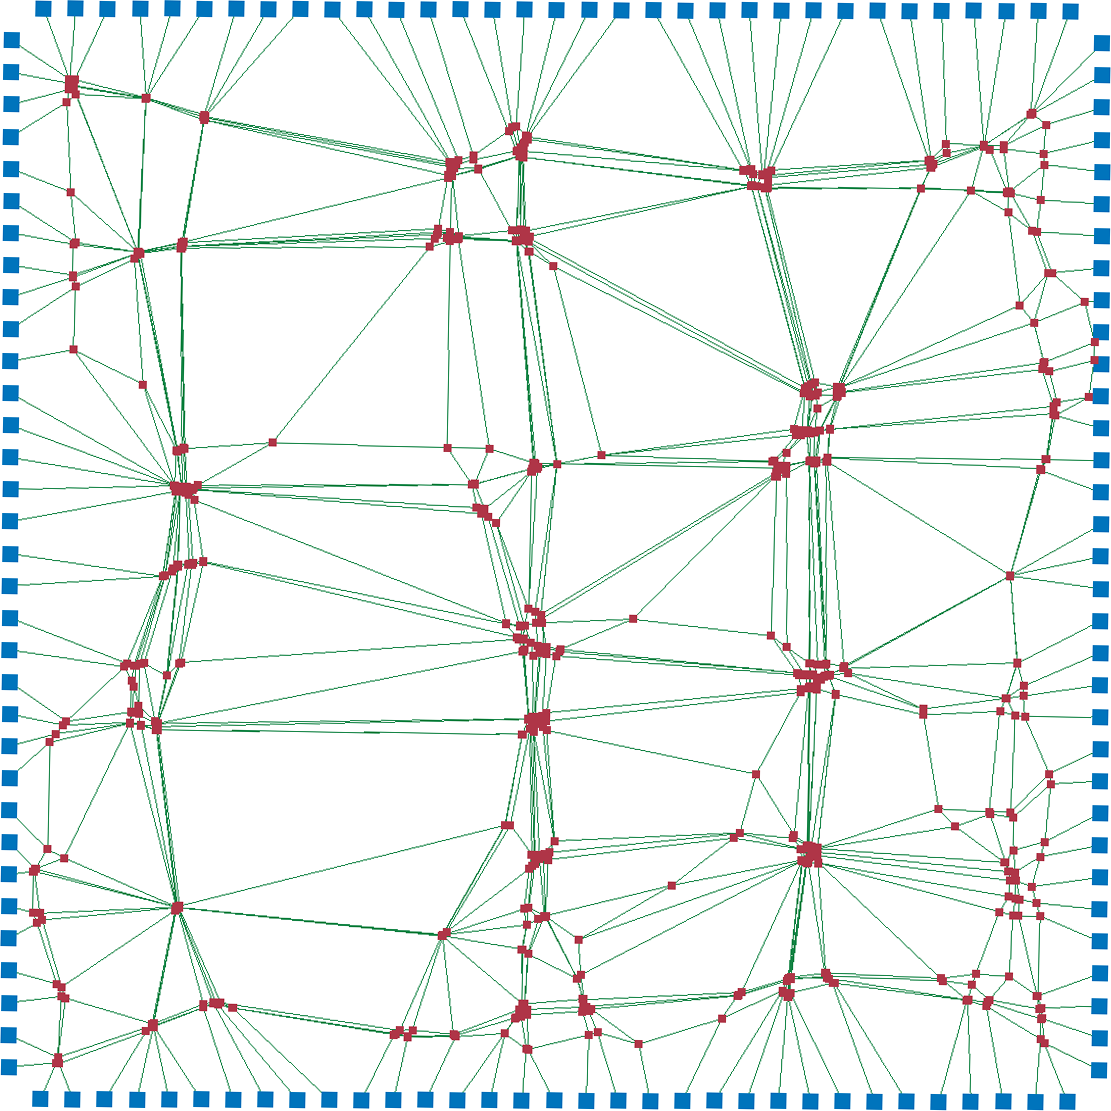
\includegraphics[
		width=\textwidth, 
		height=\textwidth, 
		keepaspectratio=true]
	{./img/results/1200_0_1_stretchHighest_97_step_100}
	\caption{Step 100}
	\label{fig:experiment:stretchHighestStrain:100}
\end{subfigure}					
		\caption{Several steps of the simulation where at each step where springs are stretched the springs with a strain greater than 1.04 are stretched.}
		\label{fig:experiment:stretchHighest}
	\end{figure*}
	\todo[inline]{Discuss results of stretching springs with strain greater than.}


% Discuss influence of parameters
% Number
\todo[inline]{Number of springs to break: Uitzonderingen wroden niet goed afgehandled}
\todo[inline]{Number of springs to break: Hoe relateert het aantal dat je breekt aan de rest van de simulatie?}
\todo[inline]{Number of springs to break: Wat is het effect van hoge/lage waarden}

% Strain
\todo[inline]{Strain threshold: De strain zou aangepast moeten worden naarmate de simulatie vordert, zodat de modder nooit klaar is met opdrogen?}
\todo[inline]{Strain threshold: Wat is het effect van hoge/lage waarden}

% Stretch factor
\todo[inline]{Stretch factor: Wat betekent een hogere/lagere stretch factor voor het materiaal?}
\todo[inline]{Stretch factor: Wat is het effect van hoge/lage waarden}